\documentclass[a4paper]{book}
\usepackage{a4wide}
\usepackage{makeidx}
\usepackage{graphicx}
\usepackage{multicol}
\usepackage{float}
\usepackage{listings}
\usepackage{color}
\usepackage{textcomp}
\usepackage{alltt}
\usepackage{times}
\usepackage{ifpdf}
\ifpdf
\usepackage[pdftex,
            pagebackref=true,
            colorlinks=true,
            linkcolor=blue,
            unicode
           ]{hyperref}
\else
\usepackage[ps2pdf,
            pagebackref=true,
            colorlinks=true,
            linkcolor=blue,
            unicode
           ]{hyperref}
\usepackage{pspicture}
\fi
\usepackage[utf8]{inputenc}
\usepackage{doxygen}
\lstset{language=C++,inputencoding=utf8,basicstyle=\footnotesize,breaklines=true,breakatwhitespace=true,tabsize=8,numbers=left }
\makeindex
\setcounter{tocdepth}{3}
\renewcommand{\footrulewidth}{0.4pt}
\begin{document}
\hypersetup{pageanchor=false}
\begin{titlepage}
\vspace*{7cm}
\begin{center}
{\Large Shopped \\[1ex]\large Iteration 3 }\\
\vspace*{1cm}
{\large Generated by Doxygen 1.6.1}\\
\vspace*{0.5cm}
{\small Mon Oct 26 20:11:45 2009}\\
\end{center}
\end{titlepage}
\clearemptydoublepage
\pagenumbering{roman}
\tableofcontents
\clearemptydoublepage
\pagenumbering{arabic}
\hypersetup{pageanchor=true}
\chapter{Namespace Index}
\section{Namespace List}
Here is a list of all namespaces with brief descriptions:\begin{DoxyCompactList}
\item\contentsline{section}{\hyperlink{namespace_core}{Core} }{\pageref{namespace_core}}{}
\item\contentsline{section}{\hyperlink{namespace_core_1_1_images}{Core::Images} }{\pageref{namespace_core_1_1_images}}{}
\item\contentsline{section}{\hyperlink{namespace_core_1_1_interfaces}{Core::Interfaces} }{\pageref{namespace_core_1_1_interfaces}}{}
\item\contentsline{section}{\hyperlink{namespace_tests}{Tests} }{\pageref{namespace_tests}}{}
\item\contentsline{section}{\hyperlink{namespace_u_i}{UI} }{\pageref{namespace_u_i}}{}
\item\contentsline{section}{\hyperlink{namespace_u_i_1_1_properties}{UI::Properties} }{\pageref{namespace_u_i_1_1_properties}}{}
\end{DoxyCompactList}

\chapter{Class Index}
\section{Class Hierarchy}
This inheritance list is sorted roughly, but not completely, alphabetically:\begin{DoxyCompactList}
\item \contentsline{section}{Core.Images.CurrentImage}{\pageref{class_core_1_1_images_1_1_current_image}}{}
\item \contentsline{section}{Core.Interfaces.IFileOperations}{\pageref{interface_core_1_1_interfaces_1_1_i_file_operations}}{}
\begin{DoxyCompactList}
\item \contentsline{section}{Core.FileOperations}{\pageref{class_core_1_1_file_operations}}{}
\end{DoxyCompactList}
\item \contentsline{section}{Core.ImageRotate}{\pageref{class_core_1_1_image_rotate}}{}
\item \contentsline{section}{UI.Properties.Resources}{\pageref{class_u_i_1_1_properties_1_1_resources}}{}
\item \contentsline{section}{UI.RotateDialog}{\pageref{class_u_i_1_1_rotate_dialog}}{}
\item \contentsline{section}{UI.Properties.Settings}{\pageref{class_u_i_1_1_properties_1_1_settings}}{}
\item \contentsline{section}{UI.ShoppedGui}{\pageref{class_u_i_1_1_shopped_gui}}{}
\end{DoxyCompactList}

\chapter{Class Index}
\section{Class List}
Here are the classes, structs, unions and interfaces with brief descriptions:\begin{DoxyCompactList}
\item\contentsline{section}{\hyperlink{class_core_1_1_images_1_1_current_image}{Core::Images::CurrentImage} }{\pageref{class_core_1_1_images_1_1_current_image}}{}
\item\contentsline{section}{\hyperlink{class_core_1_1_file_operations}{Core::FileOperations} }{\pageref{class_core_1_1_file_operations}}{}
\item\contentsline{section}{\hyperlink{interface_core_1_1_interfaces_1_1_i_file_operations}{Core::Interfaces::IFileOperations} }{\pageref{interface_core_1_1_interfaces_1_1_i_file_operations}}{}
\item\contentsline{section}{\hyperlink{class_core_1_1_image_rotate}{Core::ImageRotate} }{\pageref{class_core_1_1_image_rotate}}{}
\item\contentsline{section}{\hyperlink{class_u_i_1_1_resize_dialog}{UI::ResizeDialog} }{\pageref{class_u_i_1_1_resize_dialog}}{}
\item\contentsline{section}{\hyperlink{class_u_i_1_1_properties_1_1_resources}{UI::Properties::Resources} (A strongly-\/typed resource class, for looking up localized strings, etc )}{\pageref{class_u_i_1_1_properties_1_1_resources}}{}
\item\contentsline{section}{\hyperlink{class_u_i_1_1_rotate_dialog}{UI::RotateDialog} }{\pageref{class_u_i_1_1_rotate_dialog}}{}
\item\contentsline{section}{\hyperlink{class_u_i_1_1_properties_1_1_settings}{UI::Properties::Settings} }{\pageref{class_u_i_1_1_properties_1_1_settings}}{}
\item\contentsline{section}{\hyperlink{class_u_i_1_1_shopped_gui}{UI::ShoppedGui} }{\pageref{class_u_i_1_1_shopped_gui}}{}
\item\contentsline{section}{\hyperlink{class_u_i_1_1_zoom_dialog}{UI::ZoomDialog} }{\pageref{class_u_i_1_1_zoom_dialog}}{}
\end{DoxyCompactList}

\chapter{File Index}
\section{File List}
Here is a list of all files with brief descriptions:\begin{DoxyCompactList}
\item\contentsline{section}{C:/Users/Andy/Documents/Visual Studio 2008/Projects/capstone2009/shopped/Core/\hyperlink{_file_operations_8cs}{FileOperations.cs} }{\pageref{_file_operations_8cs}}{}
\item\contentsline{section}{C:/Users/Andy/Documents/Visual Studio 2008/Projects/capstone2009/shopped/Core/\hyperlink{_grayscale_8cs}{Grayscale.cs} }{\pageref{_grayscale_8cs}}{}
\item\contentsline{section}{C:/Users/Andy/Documents/Visual Studio 2008/Projects/capstone2009/shopped/Core/\hyperlink{_image_history_8cs}{ImageHistory.cs} }{\pageref{_image_history_8cs}}{}
\item\contentsline{section}{C:/Users/Andy/Documents/Visual Studio 2008/Projects/capstone2009/shopped/Core/\hyperlink{_image_history_item_8cs}{ImageHistoryItem.cs} }{\pageref{_image_history_item_8cs}}{}
\item\contentsline{section}{C:/Users/Andy/Documents/Visual Studio 2008/Projects/capstone2009/shopped/Core/\hyperlink{_image_resize_8cs}{ImageResize.cs} }{\pageref{_image_resize_8cs}}{}
\item\contentsline{section}{C:/Users/Andy/Documents/Visual Studio 2008/Projects/capstone2009/shopped/Core/\hyperlink{_image_rotate_8cs}{ImageRotate.cs} }{\pageref{_image_rotate_8cs}}{}
\item\contentsline{section}{C:/Users/Andy/Documents/Visual Studio 2008/Projects/capstone2009/shopped/Core/\hyperlink{_image_zoom_8cs}{ImageZoom.cs} }{\pageref{_image_zoom_8cs}}{}
\item\contentsline{section}{C:/Users/Andy/Documents/Visual Studio 2008/Projects/capstone2009/shopped/Core/\hyperlink{_shopped_gui_helper_8cs}{ShoppedGuiHelper.cs} }{\pageref{_shopped_gui_helper_8cs}}{}
\item\contentsline{section}{C:/Users/Andy/Documents/Visual Studio 2008/Projects/capstone2009/shopped/Core/Images/\hyperlink{_picture_box_image_8cs}{PictureBoxImage.cs} }{\pageref{_picture_box_image_8cs}}{}
\item\contentsline{section}{C:/Users/Andy/Documents/Visual Studio 2008/Projects/capstone2009/shopped/Core/Interfaces/\hyperlink{_i_file_operations_8cs}{IFileOperations.cs} }{\pageref{_i_file_operations_8cs}}{}
\item\contentsline{section}{C:/Users/Andy/Documents/Visual Studio 2008/Projects/capstone2009/shopped/Core/Properties/\hyperlink{_core_2_properties_2_assembly_info_8cs}{AssemblyInfo.cs} }{\pageref{_core_2_properties_2_assembly_info_8cs}}{}
\item\contentsline{section}{C:/Users/Andy/Documents/Visual Studio 2008/Projects/capstone2009/shopped/Tests/\hyperlink{_image_resize_tester_8cs}{ImageResizeTester.cs} }{\pageref{_image_resize_tester_8cs}}{}
\item\contentsline{section}{C:/Users/Andy/Documents/Visual Studio 2008/Projects/capstone2009/shopped/Tests/\hyperlink{_image_rotate_tester_8cs}{ImageRotateTester.cs} }{\pageref{_image_rotate_tester_8cs}}{}
\item\contentsline{section}{C:/Users/Andy/Documents/Visual Studio 2008/Projects/capstone2009/shopped/Tests/\hyperlink{_image_zoom_tester_8cs}{ImageZoomTester.cs} }{\pageref{_image_zoom_tester_8cs}}{}
\item\contentsline{section}{C:/Users/Andy/Documents/Visual Studio 2008/Projects/capstone2009/shopped/Tests/\hyperlink{_picture_box_image_tester_8cs}{PictureBoxImageTester.cs} }{\pageref{_picture_box_image_tester_8cs}}{}
\item\contentsline{section}{C:/Users/Andy/Documents/Visual Studio 2008/Projects/capstone2009/shopped/Tests/Properties/\hyperlink{_tests_2_properties_2_assembly_info_8cs}{AssemblyInfo.cs} }{\pageref{_tests_2_properties_2_assembly_info_8cs}}{}
\item\contentsline{section}{C:/Users/Andy/Documents/Visual Studio 2008/Projects/capstone2009/shopped/UI/\hyperlink{_program_8cs}{Program.cs} }{\pageref{_program_8cs}}{}
\item\contentsline{section}{C:/Users/Andy/Documents/Visual Studio 2008/Projects/capstone2009/shopped/UI/\hyperlink{_resize_dialog_8cs}{ResizeDialog.cs} }{\pageref{_resize_dialog_8cs}}{}
\item\contentsline{section}{C:/Users/Andy/Documents/Visual Studio 2008/Projects/capstone2009/shopped/UI/\hyperlink{_resize_dialog_8_designer_8cs}{ResizeDialog.Designer.cs} }{\pageref{_resize_dialog_8_designer_8cs}}{}
\item\contentsline{section}{C:/Users/Andy/Documents/Visual Studio 2008/Projects/capstone2009/shopped/UI/\hyperlink{_rotate_dialog_8cs}{RotateDialog.cs} }{\pageref{_rotate_dialog_8cs}}{}
\item\contentsline{section}{C:/Users/Andy/Documents/Visual Studio 2008/Projects/capstone2009/shopped/UI/\hyperlink{_rotate_dialog_8_designer_8cs}{RotateDialog.Designer.cs} }{\pageref{_rotate_dialog_8_designer_8cs}}{}
\item\contentsline{section}{C:/Users/Andy/Documents/Visual Studio 2008/Projects/capstone2009/shopped/UI/\hyperlink{_shopped_gui_8cs}{ShoppedGui.cs} }{\pageref{_shopped_gui_8cs}}{}
\item\contentsline{section}{C:/Users/Andy/Documents/Visual Studio 2008/Projects/capstone2009/shopped/UI/\hyperlink{_shopped_gui_8_designer_8cs}{ShoppedGui.Designer.cs} }{\pageref{_shopped_gui_8_designer_8cs}}{}
\item\contentsline{section}{C:/Users/Andy/Documents/Visual Studio 2008/Projects/capstone2009/shopped/UI/\hyperlink{_zoom_dialog_8cs}{ZoomDialog.cs} }{\pageref{_zoom_dialog_8cs}}{}
\item\contentsline{section}{C:/Users/Andy/Documents/Visual Studio 2008/Projects/capstone2009/shopped/UI/\hyperlink{_zoom_dialog_8_designer_8cs}{ZoomDialog.Designer.cs} }{\pageref{_zoom_dialog_8_designer_8cs}}{}
\item\contentsline{section}{C:/Users/Andy/Documents/Visual Studio 2008/Projects/capstone2009/shopped/UI/Properties/\hyperlink{_u_i_2_properties_2_assembly_info_8cs}{AssemblyInfo.cs} }{\pageref{_u_i_2_properties_2_assembly_info_8cs}}{}
\item\contentsline{section}{C:/Users/Andy/Documents/Visual Studio 2008/Projects/capstone2009/shopped/UI/Properties/\hyperlink{_resources_8_designer_8cs}{Resources.Designer.cs} }{\pageref{_resources_8_designer_8cs}}{}
\item\contentsline{section}{C:/Users/Andy/Documents/Visual Studio 2008/Projects/capstone2009/shopped/UI/Properties/\hyperlink{_settings_8_designer_8cs}{Settings.Designer.cs} }{\pageref{_settings_8_designer_8cs}}{}
\end{DoxyCompactList}

\chapter{Namespace Documentation}
\hypertarget{namespace_core}{
\section{Core Namespace Reference}
\label{namespace_core}\index{Core@{Core}}
}
\subsection*{Namespaces}
\begin{DoxyCompactItemize}
\item 
namespace \hyperlink{namespace_core_1_1_images}{Images}
\item 
namespace \hyperlink{namespace_core_1_1_interfaces}{Interfaces}
\end{DoxyCompactItemize}
\subsection*{Classes}
\begin{DoxyCompactItemize}
\item 
class \hyperlink{class_core_1_1_file_operations}{FileOperations}
\item 
class \hyperlink{class_core_1_1_grayscale}{Grayscale}
\item 
class \hyperlink{class_core_1_1_image_history}{ImageHistory}
\item 
class \hyperlink{class_core_1_1_image_history_item}{ImageHistoryItem}
\item 
class \hyperlink{class_core_1_1_image_resize}{ImageResize}
\item 
class \hyperlink{class_core_1_1_image_rotate}{ImageRotate}
\item 
class \hyperlink{class_core_1_1_image_zoom}{ImageZoom}
\item 
class \hyperlink{class_core_1_1_shopped_gui_helper}{ShoppedGuiHelper}
\end{DoxyCompactItemize}

\hypertarget{namespace_core_1_1_images}{
\section{Core::Images Namespace Reference}
\label{namespace_core_1_1_images}\index{Core::Images@{Core::Images}}
}
\subsection*{Classes}
\begin{DoxyCompactItemize}
\item 
class \hyperlink{class_core_1_1_images_1_1_picture_box_image}{PictureBoxImage}
\end{DoxyCompactItemize}

\hypertarget{namespace_core_1_1_interfaces}{
\section{Core::Interfaces Namespace Reference}
\label{namespace_core_1_1_interfaces}\index{Core::Interfaces@{Core::Interfaces}}
}
\subsection*{Classes}
\begin{DoxyCompactItemize}
\item 
interface \hyperlink{interface_core_1_1_interfaces_1_1_i_file_operations}{IFileOperations}
\end{DoxyCompactItemize}

\hypertarget{namespace_tests}{
\section{Tests Namespace Reference}
\label{namespace_tests}\index{Tests@{Tests}}
}
\subsection*{Classes}
\begin{DoxyCompactItemize}
\item 
class \hyperlink{class_tests_1_1_image_resize_tester}{ImageResizeTester}
\item 
class \hyperlink{class_tests_1_1_image_rotate_tester}{ImageRotateTester}
\item 
class \hyperlink{class_tests_1_1_image_zoom_tester}{ImageZoomTester}
\item 
class \hyperlink{class_tests_1_1_picture_box_image_tester}{PictureBoxImageTester}
\end{DoxyCompactItemize}

\hypertarget{namespace_u_i}{
\section{UI Namespace Reference}
\label{namespace_u_i}\index{UI@{UI}}
}
\subsection*{Namespaces}
\begin{DoxyCompactItemize}
\item 
namespace \hyperlink{namespace_u_i_1_1_properties}{Properties}
\end{DoxyCompactItemize}
\subsection*{Classes}
\begin{DoxyCompactItemize}
\item 
class \hyperlink{class_u_i_1_1_program}{Program}
\item 
class \hyperlink{class_u_i_1_1_resize_dialog}{ResizeDialog}
\item 
class \hyperlink{class_u_i_1_1_rotate_dialog}{RotateDialog}
\item 
class \hyperlink{class_u_i_1_1_shopped_gui}{ShoppedGui}
\item 
class \hyperlink{class_u_i_1_1_zoom_dialog}{ZoomDialog}
\end{DoxyCompactItemize}

\hypertarget{namespace_u_i_1_1_properties}{
\section{UI::Properties Namespace Reference}
\label{namespace_u_i_1_1_properties}\index{UI::Properties@{UI::Properties}}
}
\subsection*{Classes}
\begin{DoxyCompactItemize}
\item 
class \hyperlink{class_u_i_1_1_properties_1_1_resources}{Resources}
\begin{DoxyCompactList}\small\item\em A strongly-\/typed resource class, for looking up localized strings, etc. \item\end{DoxyCompactList}\item 
class \hyperlink{class_u_i_1_1_properties_1_1_settings}{Settings}
\end{DoxyCompactItemize}

\chapter{Class Documentation}
\hypertarget{class_core_1_1_file_operations}{
\section{Core::FileOperations Class Reference}
\label{class_core_1_1_file_operations}\index{Core::FileOperations@{Core::FileOperations}}
}
Inheritance diagram for Core::FileOperations::\begin{figure}[H]
\begin{center}
\leavevmode
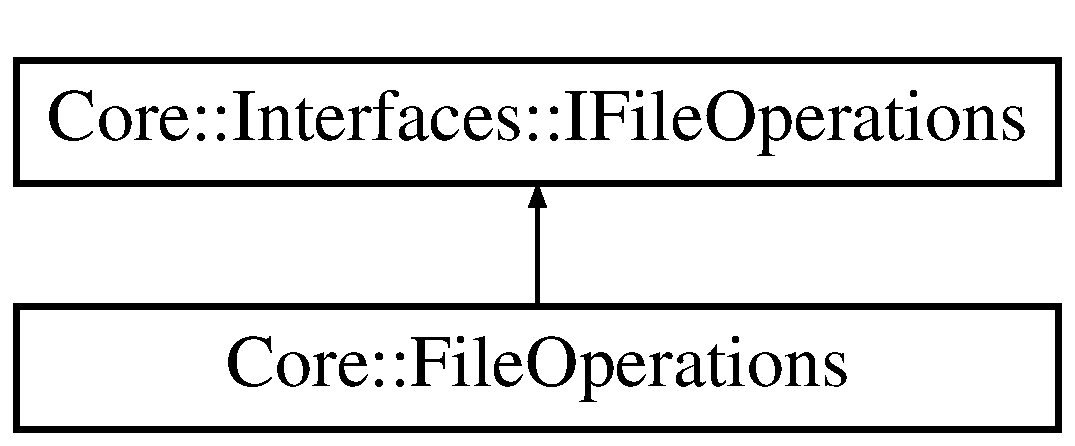
\includegraphics[height=2cm]{class_core_1_1_file_operations}
\end{center}
\end{figure}
\subsection*{Public Member Functions}
\begin{DoxyCompactItemize}
\item 
string \hyperlink{class_core_1_1_file_operations_a23fa84c311fb8051caa8e751d99ef027}{OpenFile} (ref Image imageToOpen)
\item 
void \hyperlink{class_core_1_1_file_operations_a4437acc296a0a32cdf8727ef5a7e94ce}{SaveFile} (Image imageToSave, string fileCurrentlyOpen)
\end{DoxyCompactItemize}


\subsection{Member Function Documentation}
\hypertarget{class_core_1_1_file_operations_a23fa84c311fb8051caa8e751d99ef027}{
\index{Core::FileOperations@{Core::FileOperations}!OpenFile@{OpenFile}}
\index{OpenFile@{OpenFile}!Core::FileOperations@{Core::FileOperations}}
\subsubsection[{OpenFile}]{\setlength{\rightskip}{0pt plus 5cm}string Core::FileOperations::OpenFile (ref Image {\em imageToOpen})\hspace{0.3cm}{\ttfamily  \mbox{[}inline\mbox{]}}}}
\label{class_core_1_1_file_operations_a23fa84c311fb8051caa8e751d99ef027}
Opens a file dialog to select an image, then opens the file inside the Shopped main GUI.


\begin{DoxyParams}{Parameters}
\item[{\em imageToOpen}]This will hold the data of the opened image. \end{DoxyParams}
\begin{DoxyReturn}{Returns}
The absolute path and file name of the opened image. 
\end{DoxyReturn}


Implements \hyperlink{interface_core_1_1_interfaces_1_1_i_file_operations}{Core::Interfaces::IFileOperations}.\hypertarget{class_core_1_1_file_operations_a4437acc296a0a32cdf8727ef5a7e94ce}{
\index{Core::FileOperations@{Core::FileOperations}!SaveFile@{SaveFile}}
\index{SaveFile@{SaveFile}!Core::FileOperations@{Core::FileOperations}}
\subsubsection[{SaveFile}]{\setlength{\rightskip}{0pt plus 5cm}void Core::FileOperations::SaveFile (Image {\em imageToSave}, \/  string {\em fileCurrentlyOpen})\hspace{0.3cm}{\ttfamily  \mbox{[}inline\mbox{]}}}}
\label{class_core_1_1_file_operations_a4437acc296a0a32cdf8727ef5a7e94ce}
Opens a save file dialog to save the image that is open in the Shopped main GUI.


\begin{DoxyParams}{Parameters}
\item[{\em imageToSave}]The image that is currently open in the Shopped main GUI. \item[{\em fileCurrentlyOpen}]The absolute file path to the image that was originally opened in \hyperlink{class_core_1_1_file_operations_a23fa84c311fb8051caa8e751d99ef027}{OpenFile()} \end{DoxyParams}


Implements \hyperlink{interface_core_1_1_interfaces_1_1_i_file_operations}{Core::Interfaces::IFileOperations}.

The documentation for this class was generated from the following file:\begin{DoxyCompactItemize}
\item 
C:/Users/Andy/Documents/Visual Studio 2008/Projects/capstone2009/shopped\_\-iteration1/Core/FileOperations.cs\end{DoxyCompactItemize}

\hypertarget{class_core_1_1_grayscale}{
\section{Core::Grayscale Class Reference}
\label{class_core_1_1_grayscale}\index{Core::Grayscale@{Core::Grayscale}}
}
\subsection*{Public Member Functions}
\begin{DoxyCompactItemize}
\item 
\hyperlink{class_core_1_1_images_1_1_picture_box_image}{PictureBoxImage} \hyperlink{class_core_1_1_grayscale_aec6bcfc2f573c3a24e896a08e06468a3}{MakeGrayscale} (\hyperlink{class_core_1_1_images_1_1_picture_box_image}{PictureBoxImage} pictureBoxImage)
\end{DoxyCompactItemize}


\subsection{Member Function Documentation}
\hypertarget{class_core_1_1_grayscale_aec6bcfc2f573c3a24e896a08e06468a3}{
\index{Core::Grayscale@{Core::Grayscale}!MakeGrayscale@{MakeGrayscale}}
\index{MakeGrayscale@{MakeGrayscale}!Core::Grayscale@{Core::Grayscale}}
\subsubsection[{MakeGrayscale}]{\setlength{\rightskip}{0pt plus 5cm}{\bf PictureBoxImage} Core::Grayscale::MakeGrayscale ({\bf PictureBoxImage} {\em pictureBoxImage})\hspace{0.3cm}{\ttfamily  \mbox{[}inline\mbox{]}}}}
\label{class_core_1_1_grayscale_aec6bcfc2f573c3a24e896a08e06468a3}
A filter that will make an Image object grayscale.


\begin{DoxyParams}{Parameters}
\item[{\em pictureBoxImage}]The PictureBoxImage object in the current context of Shopped GUI \end{DoxyParams}
\begin{DoxyReturn}{Returns}
A PictureBoxImage object with the appropriate properties set by this method. 
\end{DoxyReturn}


The documentation for this class was generated from the following file:\begin{DoxyCompactItemize}
\item 
C:/Users/Andy/Documents/Visual Studio 2008/Projects/capstone2009/shopped/Core/\hyperlink{_grayscale_8cs}{Grayscale.cs}\end{DoxyCompactItemize}

\hypertarget{interface_core_1_1_interfaces_1_1_i_file_operations}{
\section{Core::Interfaces::IFileOperations Interface Reference}
\label{interface_core_1_1_interfaces_1_1_i_file_operations}\index{Core::Interfaces::IFileOperations@{Core::Interfaces::IFileOperations}}
}
Inheritance diagram for Core::Interfaces::IFileOperations::\begin{figure}[H]
\begin{center}
\leavevmode
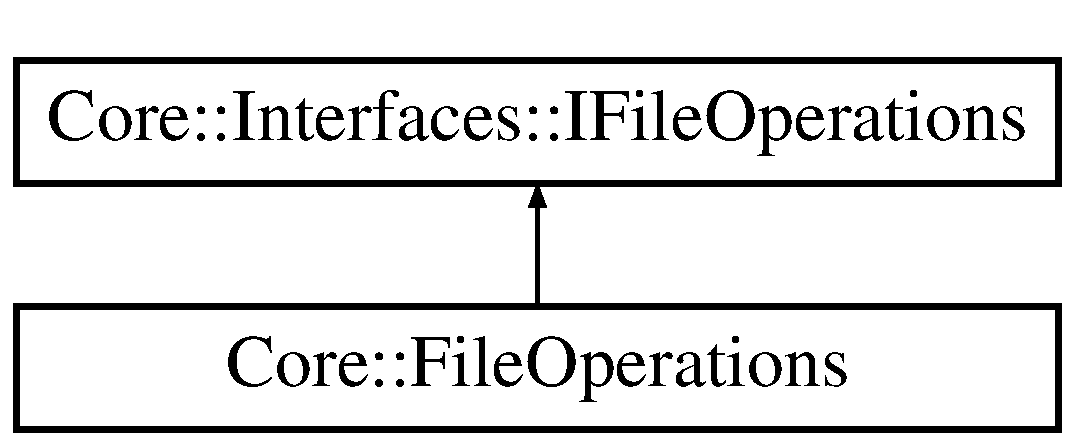
\includegraphics[height=2cm]{interface_core_1_1_interfaces_1_1_i_file_operations}
\end{center}
\end{figure}
\subsection*{Public Member Functions}
\begin{DoxyCompactItemize}
\item 
\hyperlink{class_core_1_1_images_1_1_picture_box_image}{PictureBoxImage} \hyperlink{interface_core_1_1_interfaces_1_1_i_file_operations_a373c3e1cc40a59b65e77cf9551463419}{OpenFile} (\hyperlink{class_core_1_1_images_1_1_picture_box_image}{PictureBoxImage} pictureBoxImage)
\item 
void \hyperlink{interface_core_1_1_interfaces_1_1_i_file_operations_a254301628fd3053115f557626aa71f14}{SaveFile} (\hyperlink{class_core_1_1_images_1_1_picture_box_image}{PictureBoxImage} pictureBoxImage)
\end{DoxyCompactItemize}


\subsection{Detailed Description}
\hyperlink{interface_core_1_1_interfaces_1_1_i_file_operations}{IFileOperations} is an interface to the \hyperlink{class_core_1_1_file_operations}{FileOperations} class. The interface contains two methods, OpenFile and SaveFile. 

\subsection{Member Function Documentation}
\hypertarget{interface_core_1_1_interfaces_1_1_i_file_operations_a373c3e1cc40a59b65e77cf9551463419}{
\index{Core::Interfaces::IFileOperations@{Core::Interfaces::IFileOperations}!OpenFile@{OpenFile}}
\index{OpenFile@{OpenFile}!Core::Interfaces::IFileOperations@{Core::Interfaces::IFileOperations}}
\subsubsection[{OpenFile}]{\setlength{\rightskip}{0pt plus 5cm}{\bf PictureBoxImage} Core::Interfaces::IFileOperations::OpenFile ({\bf PictureBoxImage} {\em pictureBoxImage})}}
\label{interface_core_1_1_interfaces_1_1_i_file_operations_a373c3e1cc40a59b65e77cf9551463419}


Implemented in \hyperlink{class_core_1_1_file_operations_a108130b2bd87d432c0fbbb4f6a42c662}{Core::FileOperations}.\hypertarget{interface_core_1_1_interfaces_1_1_i_file_operations_a254301628fd3053115f557626aa71f14}{
\index{Core::Interfaces::IFileOperations@{Core::Interfaces::IFileOperations}!SaveFile@{SaveFile}}
\index{SaveFile@{SaveFile}!Core::Interfaces::IFileOperations@{Core::Interfaces::IFileOperations}}
\subsubsection[{SaveFile}]{\setlength{\rightskip}{0pt plus 5cm}void Core::Interfaces::IFileOperations::SaveFile ({\bf PictureBoxImage} {\em pictureBoxImage})}}
\label{interface_core_1_1_interfaces_1_1_i_file_operations_a254301628fd3053115f557626aa71f14}


Implemented in \hyperlink{class_core_1_1_file_operations_a0fc5427e96d79e70c6409ec22e70abba}{Core::FileOperations}.

The documentation for this interface was generated from the following file:\begin{DoxyCompactItemize}
\item 
C:/Users/Andy/Documents/Visual Studio 2008/Projects/capstone2009/shopped/Core/Interfaces/\hyperlink{_i_file_operations_8cs}{IFileOperations.cs}\end{DoxyCompactItemize}

\hypertarget{class_core_1_1_image_history}{
\section{Core::ImageHistory Class Reference}
\label{class_core_1_1_image_history}\index{Core::ImageHistory@{Core::ImageHistory}}
}
\subsection*{Public Member Functions}
\begin{DoxyCompactItemize}
\item 
void \hyperlink{class_core_1_1_image_history_a6631d7fefea3a1a28fc6dcdf887daf37}{AddImageToImageHistory} (Image image, string operation)
\item 
Image \hyperlink{class_core_1_1_image_history_ade2a92df5f5525b0e3951b45b2f3434e}{Undo} ()
\item 
Image \hyperlink{class_core_1_1_image_history_afc601ae64181e745d9d94f4b16633a90}{Redo} ()
\item 
int \hyperlink{class_core_1_1_image_history_ae26bcfeed34a733dd372896a86bbc3d4}{GetNumberOfImagesInHistory} ()
\item 
int \hyperlink{class_core_1_1_image_history_a421e672ff9f20e10a03bf989cff4442e}{GetCurrentRevision} ()
\end{DoxyCompactItemize}
\subsection*{Public Attributes}
\begin{DoxyCompactItemize}
\item 
\hypertarget{class_core_1_1_image_history_abb81d12e0bcf3f1f0e79c797f38cc6f2}{
List$<$ \hyperlink{class_core_1_1_image_history_item}{ImageHistoryItem} $>$ {\bfseries ImageRevisions}}
\label{class_core_1_1_image_history_abb81d12e0bcf3f1f0e79c797f38cc6f2}

\end{DoxyCompactItemize}
\subsection*{Private Attributes}
\begin{DoxyCompactItemize}
\item 
\hypertarget{class_core_1_1_image_history_a1a695f64608fc10b95bce32634092f3c}{
int {\bfseries CurrentRevision}}
\label{class_core_1_1_image_history_a1a695f64608fc10b95bce32634092f3c}

\end{DoxyCompactItemize}


\subsection{Detailed Description}
Manages the list of ImageHistoryItems (to do undo and redo) as well as carry out the undo and redo operations. 
\begin{DoxyParams}{Parameters}
\item[{\em ImageRevisions}]A list of \hyperlink{class_core_1_1_image_history_item}{ImageHistoryItem} objects (which contain an Image object and a string detailing the operation). \end{DoxyParams}


\subsection{Member Function Documentation}
\hypertarget{class_core_1_1_image_history_a6631d7fefea3a1a28fc6dcdf887daf37}{
\index{Core::ImageHistory@{Core::ImageHistory}!AddImageToImageHistory@{AddImageToImageHistory}}
\index{AddImageToImageHistory@{AddImageToImageHistory}!Core::ImageHistory@{Core::ImageHistory}}
\subsubsection[{AddImageToImageHistory}]{\setlength{\rightskip}{0pt plus 5cm}void Core::ImageHistory::AddImageToImageHistory (Image {\em image}, \/  string {\em operation})\hspace{0.3cm}{\ttfamily  \mbox{[}inline\mbox{]}}}}
\label{class_core_1_1_image_history_a6631d7fefea3a1a28fc6dcdf887daf37}
Appends the Image object and string passed in to the end of the ImageRevisions list. 
\begin{DoxyParams}{Parameters}
\item[{\em image}]The image to add to the list \item[{\em operation}]A string detailing what operation was just performed \end{DoxyParams}
\hypertarget{class_core_1_1_image_history_a421e672ff9f20e10a03bf989cff4442e}{
\index{Core::ImageHistory@{Core::ImageHistory}!GetCurrentRevision@{GetCurrentRevision}}
\index{GetCurrentRevision@{GetCurrentRevision}!Core::ImageHistory@{Core::ImageHistory}}
\subsubsection[{GetCurrentRevision}]{\setlength{\rightskip}{0pt plus 5cm}int Core::ImageHistory::GetCurrentRevision ()\hspace{0.3cm}{\ttfamily  \mbox{[}inline\mbox{]}}}}
\label{class_core_1_1_image_history_a421e672ff9f20e10a03bf989cff4442e}
Returns the value of the iterator (essentially where we are in the ImageRevisions list). \begin{DoxyReturn}{Returns}
CurrentRevision The value of the iterator for the list. 
\end{DoxyReturn}
\hypertarget{class_core_1_1_image_history_ae26bcfeed34a733dd372896a86bbc3d4}{
\index{Core::ImageHistory@{Core::ImageHistory}!GetNumberOfImagesInHistory@{GetNumberOfImagesInHistory}}
\index{GetNumberOfImagesInHistory@{GetNumberOfImagesInHistory}!Core::ImageHistory@{Core::ImageHistory}}
\subsubsection[{GetNumberOfImagesInHistory}]{\setlength{\rightskip}{0pt plus 5cm}int Core::ImageHistory::GetNumberOfImagesInHistory ()\hspace{0.3cm}{\ttfamily  \mbox{[}inline\mbox{]}}}}
\label{class_core_1_1_image_history_ae26bcfeed34a733dd372896a86bbc3d4}
Returns the number of \hyperlink{class_core_1_1_image_history_item}{ImageHistoryItem} objects on the ImageRevisions list. \begin{DoxyReturn}{Returns}
ImageRevisions.Count() The current number of items in the list. 
\end{DoxyReturn}
\hypertarget{class_core_1_1_image_history_afc601ae64181e745d9d94f4b16633a90}{
\index{Core::ImageHistory@{Core::ImageHistory}!Redo@{Redo}}
\index{Redo@{Redo}!Core::ImageHistory@{Core::ImageHistory}}
\subsubsection[{Redo}]{\setlength{\rightskip}{0pt plus 5cm}Image Core::ImageHistory::Redo ()\hspace{0.3cm}{\ttfamily  \mbox{[}inline\mbox{]}}}}
\label{class_core_1_1_image_history_afc601ae64181e745d9d94f4b16633a90}
Attempts a redo operation by checking if an object exists after the CurrentRevision iterator, then returning that \hyperlink{class_core_1_1_image_history_item}{ImageHistoryItem} node if it does exist. \hypertarget{class_core_1_1_image_history_ade2a92df5f5525b0e3951b45b2f3434e}{
\index{Core::ImageHistory@{Core::ImageHistory}!Undo@{Undo}}
\index{Undo@{Undo}!Core::ImageHistory@{Core::ImageHistory}}
\subsubsection[{Undo}]{\setlength{\rightskip}{0pt plus 5cm}Image Core::ImageHistory::Undo ()\hspace{0.3cm}{\ttfamily  \mbox{[}inline\mbox{]}}}}
\label{class_core_1_1_image_history_ade2a92df5f5525b0e3951b45b2f3434e}
Attempts an undo operation by checking if an object exists before the CurrentRevision iterator, then returning that \hyperlink{class_core_1_1_image_history_item}{ImageHistoryItem} node if it does exist. 

The documentation for this class was generated from the following file:\begin{DoxyCompactItemize}
\item 
C:/Users/Andy/Documents/Visual Studio 2008/Projects/capstone2009/shopped/Core/ImageHistory.cs\end{DoxyCompactItemize}

\hypertarget{class_core_1_1_image_history_item}{
\section{Core::ImageHistoryItem Class Reference}
\label{class_core_1_1_image_history_item}\index{Core::ImageHistoryItem@{Core::ImageHistoryItem}}
}
\subsection*{Properties}
\begin{DoxyCompactItemize}
\item 
\hypertarget{class_core_1_1_image_history_item_af5221965c5ea168e8ce2b248783daa23}{
Image {\bfseries Image}\hspace{0.3cm}{\ttfamily  \mbox{[}get, set\mbox{]}}}
\label{class_core_1_1_image_history_item_af5221965c5ea168e8ce2b248783daa23}

\item 
\hypertarget{class_core_1_1_image_history_item_aa0775d357dd30dafbc2de674b9bcba2b}{
string {\bfseries OperationPerformed}\hspace{0.3cm}{\ttfamily  \mbox{[}get, set\mbox{]}}}
\label{class_core_1_1_image_history_item_aa0775d357dd30dafbc2de674b9bcba2b}

\end{DoxyCompactItemize}


\subsection{Detailed Description}
A simple class that contains an Image object and a string that details the operation performed. 

The documentation for this class was generated from the following file:\begin{DoxyCompactItemize}
\item 
C:/Users/Andy/Documents/Visual Studio 2008/Projects/capstone2009/shopped/Core/ImageHistoryItem.cs\end{DoxyCompactItemize}

\hypertarget{class_core_1_1_image_resize}{
\section{Core::ImageResize Class Reference}
\label{class_core_1_1_image_resize}\index{Core::ImageResize@{Core::ImageResize}}
}
\subsection*{Public Member Functions}
\begin{DoxyCompactItemize}
\item 
void \hyperlink{class_core_1_1_image_resize_a11473ffbbb61eee829d30d3407431f67}{ResizeImage} (float resize)
\end{DoxyCompactItemize}


\subsection{Member Function Documentation}
\hypertarget{class_core_1_1_image_resize_a11473ffbbb61eee829d30d3407431f67}{
\index{Core::ImageResize@{Core::ImageResize}!ResizeImage@{ResizeImage}}
\index{ResizeImage@{ResizeImage}!Core::ImageResize@{Core::ImageResize}}
\subsubsection[{ResizeImage}]{\setlength{\rightskip}{0pt plus 5cm}void Core::ImageResize::ResizeImage (float {\em resize})\hspace{0.3cm}{\ttfamily  \mbox{[}inline\mbox{]}}}}
\label{class_core_1_1_image_resize_a11473ffbbb61eee829d30d3407431f67}
Resizes the image in the Shopped GUI to the specified resize level. 
\begin{DoxyParams}{Parameters}
\item[{\em resize}]The amount to resize the image to. \end{DoxyParams}


The documentation for this class was generated from the following file:\begin{DoxyCompactItemize}
\item 
C:/Users/Andy/Documents/Visual Studio 2008/Projects/capstone2009/shopped/Core/ImageResize.cs\end{DoxyCompactItemize}

\hypertarget{class_tests_1_1_image_resize_tester}{
\section{Tests::ImageResizeTester Class Reference}
\label{class_tests_1_1_image_resize_tester}\index{Tests::ImageResizeTester@{Tests::ImageResizeTester}}
}
\subsection*{Public Member Functions}
\begin{DoxyCompactItemize}
\item 
void \hyperlink{class_tests_1_1_image_resize_tester_a2ceceeb25362f1535aedc853a08be1d8}{ResizingImageBy200PercentDoublesSizeOfPicture} ()
\item 
void \hyperlink{class_tests_1_1_image_resize_tester_a93619ddc38161c59254054220815b0f7}{UnzoomedImageHasSamePropertiesAsCurrentImageAfterResize} ()
\end{DoxyCompactItemize}


\subsection{Member Function Documentation}
\hypertarget{class_tests_1_1_image_resize_tester_a2ceceeb25362f1535aedc853a08be1d8}{
\index{Tests::ImageResizeTester@{Tests::ImageResizeTester}!ResizingImageBy200PercentDoublesSizeOfPicture@{ResizingImageBy200PercentDoublesSizeOfPicture}}
\index{ResizingImageBy200PercentDoublesSizeOfPicture@{ResizingImageBy200PercentDoublesSizeOfPicture}!Tests::ImageResizeTester@{Tests::ImageResizeTester}}
\subsubsection[{ResizingImageBy200PercentDoublesSizeOfPicture}]{\setlength{\rightskip}{0pt plus 5cm}void Tests::ImageResizeTester::ResizingImageBy200PercentDoublesSizeOfPicture ()\hspace{0.3cm}{\ttfamily  \mbox{[}inline\mbox{]}}}}
\label{class_tests_1_1_image_resize_tester_a2ceceeb25362f1535aedc853a08be1d8}
\hypertarget{class_tests_1_1_image_resize_tester_a93619ddc38161c59254054220815b0f7}{
\index{Tests::ImageResizeTester@{Tests::ImageResizeTester}!UnzoomedImageHasSamePropertiesAsCurrentImageAfterResize@{UnzoomedImageHasSamePropertiesAsCurrentImageAfterResize}}
\index{UnzoomedImageHasSamePropertiesAsCurrentImageAfterResize@{UnzoomedImageHasSamePropertiesAsCurrentImageAfterResize}!Tests::ImageResizeTester@{Tests::ImageResizeTester}}
\subsubsection[{UnzoomedImageHasSamePropertiesAsCurrentImageAfterResize}]{\setlength{\rightskip}{0pt plus 5cm}void Tests::ImageResizeTester::UnzoomedImageHasSamePropertiesAsCurrentImageAfterResize ()\hspace{0.3cm}{\ttfamily  \mbox{[}inline\mbox{]}}}}
\label{class_tests_1_1_image_resize_tester_a93619ddc38161c59254054220815b0f7}


The documentation for this class was generated from the following file:\begin{DoxyCompactItemize}
\item 
C:/Users/Andy/Documents/Visual Studio 2008/Projects/capstone2009/shopped/Tests/\hyperlink{_image_resize_tester_8cs}{ImageResizeTester.cs}\end{DoxyCompactItemize}

\hypertarget{class_core_1_1_image_rotate}{
\section{Core.ImageRotate Class Reference}
\label{class_core_1_1_image_rotate}\index{Core::ImageRotate@{Core::ImageRotate}}
}
\subsection*{Public Member Functions}
\begin{DoxyCompactItemize}
\item 
Bitmap \hyperlink{class_core_1_1_image_rotate_afb29109d626ece8b64706820878380b4}{RotateImageByAngle} (Image image, float angle)
\end{DoxyCompactItemize}


\subsection{Member Function Documentation}
\hypertarget{class_core_1_1_image_rotate_afb29109d626ece8b64706820878380b4}{
\index{Core::ImageRotate@{Core::ImageRotate}!RotateImageByAngle@{RotateImageByAngle}}
\index{RotateImageByAngle@{RotateImageByAngle}!Core::ImageRotate@{Core::ImageRotate}}
\subsubsection[{RotateImageByAngle}]{\setlength{\rightskip}{0pt plus 5cm}Bitmap Core.ImageRotate.RotateImageByAngle (Image {\em image}, \/  float {\em angle})}}
\label{class_core_1_1_image_rotate_afb29109d626ece8b64706820878380b4}
Given a certain angle (in degrees), this method will take an image and rotate it by the given angle.


\begin{DoxyParams}{Parameters}
\item[{\em image}]The image to be rotated \item[{\em angle}]The angle (in degrees) to rotate the image \end{DoxyParams}
\begin{DoxyReturn}{Returns}
The rotated image 
\end{DoxyReturn}


The documentation for this class was generated from the following file:\begin{DoxyCompactItemize}
\item 
C:/Users/Andy/Desktop/shopped\_\-iteration1/Core/ImageRotate.cs\end{DoxyCompactItemize}

\hypertarget{class_tests_1_1_image_rotate_tester}{
\section{Tests::ImageRotateTester Class Reference}
\label{class_tests_1_1_image_rotate_tester}\index{Tests::ImageRotateTester@{Tests::ImageRotateTester}}
}
\subsection*{Public Member Functions}
\begin{DoxyCompactItemize}
\item 
void \hyperlink{class_tests_1_1_image_rotate_tester_a57ad1def77297f660af2028aeef982c9}{RotateImageSetsPictureBoxImagePropertiesToNewRotatedValues} ()
\end{DoxyCompactItemize}


\subsection{Member Function Documentation}
\hypertarget{class_tests_1_1_image_rotate_tester_a57ad1def77297f660af2028aeef982c9}{
\index{Tests::ImageRotateTester@{Tests::ImageRotateTester}!RotateImageSetsPictureBoxImagePropertiesToNewRotatedValues@{RotateImageSetsPictureBoxImagePropertiesToNewRotatedValues}}
\index{RotateImageSetsPictureBoxImagePropertiesToNewRotatedValues@{RotateImageSetsPictureBoxImagePropertiesToNewRotatedValues}!Tests::ImageRotateTester@{Tests::ImageRotateTester}}
\subsubsection[{RotateImageSetsPictureBoxImagePropertiesToNewRotatedValues}]{\setlength{\rightskip}{0pt plus 5cm}void Tests::ImageRotateTester::RotateImageSetsPictureBoxImagePropertiesToNewRotatedValues ()\hspace{0.3cm}{\ttfamily  \mbox{[}inline\mbox{]}}}}
\label{class_tests_1_1_image_rotate_tester_a57ad1def77297f660af2028aeef982c9}


The documentation for this class was generated from the following file:\begin{DoxyCompactItemize}
\item 
C:/Users/Andy/Documents/Visual Studio 2008/Projects/capstone2009/shopped/Tests/\hyperlink{_image_rotate_tester_8cs}{ImageRotateTester.cs}\end{DoxyCompactItemize}

\hypertarget{class_core_1_1_image_zoom}{
\section{Core::ImageZoom Class Reference}
\label{class_core_1_1_image_zoom}\index{Core::ImageZoom@{Core::ImageZoom}}
}
\subsection*{Public Member Functions}
\begin{DoxyCompactItemize}
\item 
void \hyperlink{class_core_1_1_image_zoom_a656d435ebf586dcec94dc46be1f46834}{ZoomImage} (float zoom)
\end{DoxyCompactItemize}


\subsection{Member Function Documentation}
\hypertarget{class_core_1_1_image_zoom_a656d435ebf586dcec94dc46be1f46834}{
\index{Core::ImageZoom@{Core::ImageZoom}!ZoomImage@{ZoomImage}}
\index{ZoomImage@{ZoomImage}!Core::ImageZoom@{Core::ImageZoom}}
\subsubsection[{ZoomImage}]{\setlength{\rightskip}{0pt plus 5cm}void Core::ImageZoom::ZoomImage (float {\em zoom})\hspace{0.3cm}{\ttfamily  \mbox{[}inline\mbox{]}}}}
\label{class_core_1_1_image_zoom_a656d435ebf586dcec94dc46be1f46834}
Zooms the image in the Shopped GUI to the specified zoom level. 
\begin{DoxyParams}{Parameters}
\item[{\em zoom}]The amount of zoom to use on the image (1.0f == 100\%). \end{DoxyParams}


The documentation for this class was generated from the following file:\begin{DoxyCompactItemize}
\item 
C:/Users/Andy/Documents/Visual Studio 2008/Projects/capstone2009/shopped/Core/ImageZoom.cs\end{DoxyCompactItemize}

\hypertarget{class_tests_1_1_image_zoom_tester}{
\section{Tests::ImageZoomTester Class Reference}
\label{class_tests_1_1_image_zoom_tester}\index{Tests::ImageZoomTester@{Tests::ImageZoomTester}}
}


The documentation for this class was generated from the following file:\begin{DoxyCompactItemize}
\item 
C:/Users/Andy/Documents/Visual Studio 2008/Projects/capstone2009/shopped/src/Tests/ImageZoomTester.cs\end{DoxyCompactItemize}

\hypertarget{class_core_1_1_images_1_1_picture_box_image}{
\section{Core::Images::PictureBoxImage Class Reference}
\label{class_core_1_1_images_1_1_picture_box_image}\index{Core::Images::PictureBoxImage@{Core::Images::PictureBoxImage}}
}
\subsection*{Public Member Functions}
\begin{DoxyCompactItemize}
\item 
\hypertarget{class_core_1_1_images_1_1_picture_box_image_a374fd6af059cb4cfd57ea034647b3f2e}{
{\bfseries PictureBoxImage} (string fileName, int height, int width, Image image)}
\label{class_core_1_1_images_1_1_picture_box_image_a374fd6af059cb4cfd57ea034647b3f2e}

\item 
\hypertarget{class_core_1_1_images_1_1_picture_box_image_ac65f665745c38330485bebdf91679618}{
{\bfseries PictureBoxImage} (\hyperlink{class_core_1_1_images_1_1_picture_box_image}{PictureBoxImage} original)}
\label{class_core_1_1_images_1_1_picture_box_image_ac65f665745c38330485bebdf91679618}

\item 
\hypertarget{class_core_1_1_images_1_1_picture_box_image_a4ad1d48954f3b11d80a2678ef1336e70}{
override string {\bfseries ToString} ()}
\label{class_core_1_1_images_1_1_picture_box_image_a4ad1d48954f3b11d80a2678ef1336e70}

\end{DoxyCompactItemize}
\subsection*{Properties}
\begin{DoxyCompactItemize}
\item 
\hypertarget{class_core_1_1_images_1_1_picture_box_image_a583e28b73d02f6f812ec97606af90633}{
string {\bfseries FileName}\hspace{0.3cm}{\ttfamily  \mbox{[}get, set\mbox{]}}}
\label{class_core_1_1_images_1_1_picture_box_image_a583e28b73d02f6f812ec97606af90633}

\item 
\hypertarget{class_core_1_1_images_1_1_picture_box_image_a104dc0c3d9d9d61336811edaf5888d46}{
int {\bfseries CurrentHeight}\hspace{0.3cm}{\ttfamily  \mbox{[}get, set\mbox{]}}}
\label{class_core_1_1_images_1_1_picture_box_image_a104dc0c3d9d9d61336811edaf5888d46}

\item 
\hypertarget{class_core_1_1_images_1_1_picture_box_image_afbb7510bda3bc049a0c9ad37b7dfcd44}{
int {\bfseries CurrentWidth}\hspace{0.3cm}{\ttfamily  \mbox{[}get, set\mbox{]}}}
\label{class_core_1_1_images_1_1_picture_box_image_afbb7510bda3bc049a0c9ad37b7dfcd44}

\item 
\hypertarget{class_core_1_1_images_1_1_picture_box_image_aa5025a4795c850b75a715596bd7cd33f}{
float {\bfseries DegreesRotated}\hspace{0.3cm}{\ttfamily  \mbox{[}get, set\mbox{]}}}
\label{class_core_1_1_images_1_1_picture_box_image_aa5025a4795c850b75a715596bd7cd33f}

\item 
\hypertarget{class_core_1_1_images_1_1_picture_box_image_a0394f492d438a5ce37f9aafa6a2c8a5b}{
float {\bfseries ZoomLevel}\hspace{0.3cm}{\ttfamily  \mbox{[}get, set\mbox{]}}}
\label{class_core_1_1_images_1_1_picture_box_image_a0394f492d438a5ce37f9aafa6a2c8a5b}

\item 
\hypertarget{class_core_1_1_images_1_1_picture_box_image_a6fce1c1aa07e08340241829db5bfa873}{
float {\bfseries ResizeLevel}\hspace{0.3cm}{\ttfamily  \mbox{[}get, set\mbox{]}}}
\label{class_core_1_1_images_1_1_picture_box_image_a6fce1c1aa07e08340241829db5bfa873}

\item 
\hypertarget{class_core_1_1_images_1_1_picture_box_image_aa0a060f15bcef8b30e629a3623386f0f}{
int {\bfseries BrightnessLevel}\hspace{0.3cm}{\ttfamily  \mbox{[}get, set\mbox{]}}}
\label{class_core_1_1_images_1_1_picture_box_image_aa0a060f15bcef8b30e629a3623386f0f}

\item 
\hypertarget{class_core_1_1_images_1_1_picture_box_image_aee6569c4f810e2e90caa9417475ac62a}{
Image {\bfseries CurrentImage}\hspace{0.3cm}{\ttfamily  \mbox{[}get, set\mbox{]}}}
\label{class_core_1_1_images_1_1_picture_box_image_aee6569c4f810e2e90caa9417475ac62a}

\end{DoxyCompactItemize}


\subsection{Detailed Description}
Holds the current state of the image in the Shopped GUI. Anytime the loaded image is modified (i.e. rotated, resized, etc.), this object gets updated to reflect the modification.


\begin{DoxyParams}{Parameters}
\item[{\em FileName}]Contains the name of the opened image file \item[{\em CurrentHeight}]Contains the height of the loaded image. \item[{\em CurrentWidth}]Contains the width of the loaded image. \item[{\em DegreesRotated}]Contains how many degrees the image is currently rotated. \item[{\em CurrentImage}]Image object that holds the actual Image object. \end{DoxyParams}


The documentation for this class was generated from the following file:\begin{DoxyCompactItemize}
\item 
C:/Users/Andy/Documents/Visual Studio 2008/Projects/capstone2009/shopped/src/Core/Images/PictureBoxImage.cs\end{DoxyCompactItemize}

\hypertarget{class_tests_1_1_picture_box_image_tester}{
\section{Tests::PictureBoxImageTester Class Reference}
\label{class_tests_1_1_picture_box_image_tester}\index{Tests::PictureBoxImageTester@{Tests::PictureBoxImageTester}}
}
\subsection*{Public Member Functions}
\begin{DoxyCompactItemize}
\item 
\hypertarget{class_tests_1_1_picture_box_image_tester_a06d878583fb2603dc081802ee581a6f2}{
void {\bfseries CanCreate} ()}
\label{class_tests_1_1_picture_box_image_tester_a06d878583fb2603dc081802ee581a6f2}

\item 
\hypertarget{class_tests_1_1_picture_box_image_tester_ac56c0c43888757c672917fe9080bac9b}{
void {\bfseries CanSetPictureBoxImageProperties} ()}
\label{class_tests_1_1_picture_box_image_tester_ac56c0c43888757c672917fe9080bac9b}

\end{DoxyCompactItemize}


The documentation for this class was generated from the following file:\begin{DoxyCompactItemize}
\item 
C:/Users/Andy/Documents/Visual Studio 2008/Projects/capstone2009/shopped/src/Tests/PictureBoxImageTester.cs\end{DoxyCompactItemize}

\hypertarget{class_u_i_1_1_program}{
\section{UI::Program Class Reference}
\label{class_u_i_1_1_program}\index{UI::Program@{UI::Program}}
}
\subsection*{Static Private Member Functions}
\begin{DoxyCompactItemize}
\item 
static void \hyperlink{class_u_i_1_1_program_a96adc9ed81265ed0455a6618d744ec8c}{Main} ()
\begin{DoxyCompactList}\small\item\em The main entry point for the application. \item\end{DoxyCompactList}\end{DoxyCompactItemize}


\subsection{Member Function Documentation}
\hypertarget{class_u_i_1_1_program_a96adc9ed81265ed0455a6618d744ec8c}{
\index{UI::Program@{UI::Program}!Main@{Main}}
\index{Main@{Main}!UI::Program@{UI::Program}}
\subsubsection[{Main}]{\setlength{\rightskip}{0pt plus 5cm}static void UI::Program::Main ()\hspace{0.3cm}{\ttfamily  \mbox{[}inline, static, private\mbox{]}}}}
\label{class_u_i_1_1_program_a96adc9ed81265ed0455a6618d744ec8c}


The main entry point for the application. 

The documentation for this class was generated from the following file:\begin{DoxyCompactItemize}
\item 
C:/Users/Andy/Documents/Visual Studio 2008/Projects/capstone2009/shopped/UI/\hyperlink{_program_8cs}{Program.cs}\end{DoxyCompactItemize}

\hypertarget{class_u_i_1_1_resize_dialog}{
\section{UI::ResizeDialog Class Reference}
\label{class_u_i_1_1_resize_dialog}\index{UI::ResizeDialog@{UI::ResizeDialog}}
}
\subsection*{Public Attributes}
\begin{DoxyCompactItemize}
\item 
\hypertarget{class_u_i_1_1_resize_dialog_af8b6b6d17d8ca70b6721793ca833f7e9}{
float {\bfseries ResizeLevel}}
\label{class_u_i_1_1_resize_dialog_af8b6b6d17d8ca70b6721793ca833f7e9}

\end{DoxyCompactItemize}
\subsection*{Private Member Functions}
\begin{DoxyCompactItemize}
\item 
void \hyperlink{class_u_i_1_1_resize_dialog_a8bd7462ff2288c8e77d91e3197729ccc}{ResizeButton\_\-Click} (object sender, EventArgs e)
\end{DoxyCompactItemize}


\subsection{Detailed Description}
The \hyperlink{class_u_i_1_1_resize_dialog}{ResizeDialog} class displays a small dialog box to prompt the user for an amount to resize the image loaded into the editor.


\begin{DoxyParams}{Parameters}
\item[{\em ResizeLevel}]Contains the amount of resize the user specifies. \end{DoxyParams}


\subsection{Member Function Documentation}
\hypertarget{class_u_i_1_1_resize_dialog_a8bd7462ff2288c8e77d91e3197729ccc}{
\index{UI::ResizeDialog@{UI::ResizeDialog}!ResizeButton\_\-Click@{ResizeButton\_\-Click}}
\index{ResizeButton\_\-Click@{ResizeButton\_\-Click}!UI::ResizeDialog@{UI::ResizeDialog}}
\subsubsection[{ResizeButton\_\-Click}]{\setlength{\rightskip}{0pt plus 5cm}void UI::ResizeDialog::ResizeButton\_\-Click (object {\em sender}, \/  EventArgs {\em e})\hspace{0.3cm}{\ttfamily  \mbox{[}inline, private\mbox{]}}}}
\label{class_u_i_1_1_resize_dialog_a8bd7462ff2288c8e77d91e3197729ccc}
Once the user hits the \char`\"{}Resize Image\char`\"{} button, this grabs the value from the dialog box. 

The documentation for this class was generated from the following file:\begin{DoxyCompactItemize}
\item 
C:/Users/Andy/Documents/Visual Studio 2008/Projects/capstone2009/shopped/UI/ResizeDialog.cs\end{DoxyCompactItemize}

\hypertarget{class_u_i_1_1_properties_1_1_resources}{
\section{UI::Properties::Resources Class Reference}
\label{class_u_i_1_1_properties_1_1_resources}\index{UI::Properties::Resources@{UI::Properties::Resources}}
}


A strongly-\/typed resource class, for looking up localized strings, etc.  
\subsection*{Properties}
\begin{DoxyCompactItemize}
\item 
static internal global::System.Resources.ResourceManager \hyperlink{class_u_i_1_1_properties_1_1_resources_a8766fbe41ebf10ebf9984cbe9e4ad7f9}{ResourceManager}\hspace{0.3cm}{\ttfamily  \mbox{[}get\mbox{]}}
\begin{DoxyCompactList}\small\item\em Returns the cached ResourceManager instance used by this class. \item\end{DoxyCompactList}\item 
static internal global::System.Globalization.CultureInfo \hyperlink{class_u_i_1_1_properties_1_1_resources_a46a0e9bbbbdb0717d4a25428483b2728}{Culture}\hspace{0.3cm}{\ttfamily  \mbox{[}get, set\mbox{]}}
\begin{DoxyCompactList}\small\item\em Overrides the current thread's CurrentUICulture property for all resource lookups using this strongly typed resource class. \item\end{DoxyCompactList}\end{DoxyCompactItemize}
\subsection*{Private Member Functions}
\begin{DoxyCompactItemize}
\item 
internal \hyperlink{class_u_i_1_1_properties_1_1_resources_aa31711d7a6220001343ebf336c8234d9}{Resources} ()
\end{DoxyCompactItemize}
\subsection*{Static Private Attributes}
\begin{DoxyCompactItemize}
\item 
static global::System.Resources.ResourceManager \hyperlink{class_u_i_1_1_properties_1_1_resources_a4d67fb5a56b27ed527034330f5614de9}{resourceMan}
\item 
static global::System.Globalization.CultureInfo \hyperlink{class_u_i_1_1_properties_1_1_resources_a25149ec96c68564c38c6537b958f98bc}{resourceCulture}
\end{DoxyCompactItemize}


\subsection{Detailed Description}
A strongly-\/typed resource class, for looking up localized strings, etc. 

\subsection{Constructor \& Destructor Documentation}
\hypertarget{class_u_i_1_1_properties_1_1_resources_aa31711d7a6220001343ebf336c8234d9}{
\index{UI::Properties::Resources@{UI::Properties::Resources}!Resources@{Resources}}
\index{Resources@{Resources}!UI::Properties::Resources@{UI::Properties::Resources}}
\subsubsection[{Resources}]{\setlength{\rightskip}{0pt plus 5cm}internal UI::Properties::Resources::Resources ()\hspace{0.3cm}{\ttfamily  \mbox{[}inline, private\mbox{]}}}}
\label{class_u_i_1_1_properties_1_1_resources_aa31711d7a6220001343ebf336c8234d9}


\subsection{Member Data Documentation}
\hypertarget{class_u_i_1_1_properties_1_1_resources_a25149ec96c68564c38c6537b958f98bc}{
\index{UI::Properties::Resources@{UI::Properties::Resources}!resourceCulture@{resourceCulture}}
\index{resourceCulture@{resourceCulture}!UI::Properties::Resources@{UI::Properties::Resources}}
\subsubsection[{resourceCulture}]{\setlength{\rightskip}{0pt plus 5cm}global::System.Globalization.CultureInfo {\bf UI::Properties::Resources::resourceCulture}\hspace{0.3cm}{\ttfamily  \mbox{[}static, private\mbox{]}}}}
\label{class_u_i_1_1_properties_1_1_resources_a25149ec96c68564c38c6537b958f98bc}
\hypertarget{class_u_i_1_1_properties_1_1_resources_a4d67fb5a56b27ed527034330f5614de9}{
\index{UI::Properties::Resources@{UI::Properties::Resources}!resourceMan@{resourceMan}}
\index{resourceMan@{resourceMan}!UI::Properties::Resources@{UI::Properties::Resources}}
\subsubsection[{resourceMan}]{\setlength{\rightskip}{0pt plus 5cm}global::System.Resources.ResourceManager {\bf UI::Properties::Resources::resourceMan}\hspace{0.3cm}{\ttfamily  \mbox{[}static, private\mbox{]}}}}
\label{class_u_i_1_1_properties_1_1_resources_a4d67fb5a56b27ed527034330f5614de9}


\subsection{Property Documentation}
\hypertarget{class_u_i_1_1_properties_1_1_resources_a46a0e9bbbbdb0717d4a25428483b2728}{
\index{UI::Properties::Resources@{UI::Properties::Resources}!Culture@{Culture}}
\index{Culture@{Culture}!UI::Properties::Resources@{UI::Properties::Resources}}
\subsubsection[{Culture}]{\setlength{\rightskip}{0pt plus 5cm}internal global::System.Globalization.CultureInfo UI::Properties::Resources::Culture\hspace{0.3cm}{\ttfamily  \mbox{[}static, get, set, private\mbox{]}}}}
\label{class_u_i_1_1_properties_1_1_resources_a46a0e9bbbbdb0717d4a25428483b2728}


Overrides the current thread's CurrentUICulture property for all resource lookups using this strongly typed resource class. \hypertarget{class_u_i_1_1_properties_1_1_resources_a8766fbe41ebf10ebf9984cbe9e4ad7f9}{
\index{UI::Properties::Resources@{UI::Properties::Resources}!ResourceManager@{ResourceManager}}
\index{ResourceManager@{ResourceManager}!UI::Properties::Resources@{UI::Properties::Resources}}
\subsubsection[{ResourceManager}]{\setlength{\rightskip}{0pt plus 5cm}internal global::System.Resources.ResourceManager UI::Properties::Resources::ResourceManager\hspace{0.3cm}{\ttfamily  \mbox{[}static, get, private\mbox{]}}}}
\label{class_u_i_1_1_properties_1_1_resources_a8766fbe41ebf10ebf9984cbe9e4ad7f9}


Returns the cached ResourceManager instance used by this class. 

The documentation for this class was generated from the following file:\begin{DoxyCompactItemize}
\item 
C:/Users/Andy/Documents/Visual Studio 2008/Projects/capstone2009/shopped/UI/Properties/\hyperlink{_resources_8_designer_8cs}{Resources.Designer.cs}\end{DoxyCompactItemize}

\hypertarget{class_u_i_1_1_rotate_dialog}{
\section{UI::RotateDialog Class Reference}
\label{class_u_i_1_1_rotate_dialog}\index{UI::RotateDialog@{UI::RotateDialog}}
}
\subsection*{Public Attributes}
\begin{DoxyCompactItemize}
\item 
\hypertarget{class_u_i_1_1_rotate_dialog_a6ea5257142dfe12543d77ab37bdf0edc}{
float {\bfseries RotateDegrees}}
\label{class_u_i_1_1_rotate_dialog_a6ea5257142dfe12543d77ab37bdf0edc}

\end{DoxyCompactItemize}


\subsection{Detailed Description}
The \hyperlink{class_u_i_1_1_rotate_dialog}{RotateDialog} class displays a small windows form to prompt the user for an amount to rotate the image loaded into the editor.


\begin{DoxyParams}{Parameters}
\item[{\em RotateDegrees}]Contains the amount of rotation (in degrees) the user specifies. \end{DoxyParams}


The documentation for this class was generated from the following file:\begin{DoxyCompactItemize}
\item 
C:/Users/Andy/Documents/Visual Studio 2008/Projects/capstone2009/shopped\_\-iteration1/UI/RotateDialog.cs\end{DoxyCompactItemize}

\hypertarget{class_u_i_1_1_properties_1_1_settings}{
\section{UI::Properties::Settings Class Reference}
\label{class_u_i_1_1_properties_1_1_settings}\index{UI::Properties::Settings@{UI::Properties::Settings}}
}
\subsection*{Properties}
\begin{DoxyCompactItemize}
\item 
\hypertarget{class_u_i_1_1_properties_1_1_settings_a15a0e6993e5dd68352a2c6f989ad5943}{
static \hyperlink{class_u_i_1_1_properties_1_1_settings}{Settings} {\bfseries Default}\hspace{0.3cm}{\ttfamily  \mbox{[}get\mbox{]}}}
\label{class_u_i_1_1_properties_1_1_settings_a15a0e6993e5dd68352a2c6f989ad5943}

\end{DoxyCompactItemize}


The documentation for this class was generated from the following file:\begin{DoxyCompactItemize}
\item 
C:/Users/Andy/Documents/Visual Studio 2008/Projects/capstone2009/shopped\_\-iteration1/UI/Properties/Settings.Designer.cs\end{DoxyCompactItemize}

\hypertarget{class_u_i_1_1_shopped_gui}{
\section{UI::ShoppedGui Class Reference}
\label{class_u_i_1_1_shopped_gui}\index{UI::ShoppedGui@{UI::ShoppedGui}}
}
\subsection*{Public Member Functions}
\begin{DoxyCompactItemize}
\item 
void \hyperlink{class_u_i_1_1_shopped_gui_a190bba777e57891c8042b86afbba83c6}{EnableGuiItems} ()
\item 
void \hyperlink{class_u_i_1_1_shopped_gui_a292a827437d7f2098c13bc1a735a569e}{SetAdditionalInfo} ()
\item 
void \hyperlink{class_u_i_1_1_shopped_gui_a3a27f074b7b204b1df148921a0dcc20c}{OpenImage} ()
\item 
void \hyperlink{class_u_i_1_1_shopped_gui_a74a1accbbc8cb69ea61830d9bfcd302c}{UpdatePictureBoxInfo} (string operation)
\item 
void \hyperlink{class_u_i_1_1_shopped_gui_a62a62fa927ca572fb7d19f8116fc8858}{SetPictureBoxOnUndo} ()
\item 
void \hyperlink{class_u_i_1_1_shopped_gui_ab6fbc914ecb121fa800ec2834daa4f37}{SetPictureBoxOnRedo} ()
\end{DoxyCompactItemize}
\subsection*{Private Member Functions}
\begin{DoxyCompactItemize}
\item 
void \hyperlink{class_u_i_1_1_shopped_gui_ad9bcb5a3a89de53a6ef580bd806fae26}{Form1\_\-Load} (object sender, EventArgs e)
\item 
void \hyperlink{class_u_i_1_1_shopped_gui_a4c3239cc225d230bafb0cc53a9f49e2c}{exitToolStripMenuItem\_\-Click} (object sender, EventArgs e)
\item 
void \hyperlink{class_u_i_1_1_shopped_gui_a04958c8af963e508601e03e14bfb8bb8}{aboutToolStripMenuItem\_\-Click} (object sender, EventArgs e)
\item 
void \hyperlink{class_u_i_1_1_shopped_gui_a5a4be38d87e3d968e9336400e572b646}{openPictureButton\_\-Click} (object sender, EventArgs e)
\item 
void \hyperlink{class_u_i_1_1_shopped_gui_a205444f0fff14792394724b4eb22601d}{saveImageButton\_\-Click} (object sender, EventArgs e)
\item 
void \hyperlink{class_u_i_1_1_shopped_gui_a059988dec5a74fcc82ee2eb503d49118}{openPictureToolStripMenuItem\_\-Click} (object sender, EventArgs e)
\item 
void \hyperlink{class_u_i_1_1_shopped_gui_a79d60e553769283f7b9ec8af7a9d3dc1}{savePictureToolStripMenuItem\_\-Click} (object sender, EventArgs e)
\item 
void \hyperlink{class_u_i_1_1_shopped_gui_a8b4824c0552bcfe814bbf8437cb87ec2}{rotateToolStripMenuItem\_\-Click} (object sender, EventArgs e)
\item 
void \hyperlink{class_u_i_1_1_shopped_gui_a5f99b03c74d01734153873d6c35fbdf3}{zoomImageToolStripMenuItem\_\-Click} (object sender, EventArgs e)
\item 
void \hyperlink{class_u_i_1_1_shopped_gui_a05e2b57477f10f88b1ee06b6b5aa4d86}{resizeToolStripMenuItem\_\-Click} (object sender, EventArgs e)
\item 
void \hyperlink{class_u_i_1_1_shopped_gui_a167624483eae61dcbe7de755ad0549a5}{undoToolStripMenuItem\_\-Click} (object sender, EventArgs e)
\item 
void \hyperlink{class_u_i_1_1_shopped_gui_a5828d5deddf5b8453e01db469a1a6f83}{redoToolStripMenuItem\_\-Click} (object sender, EventArgs e)
\item 
void \hyperlink{class_u_i_1_1_shopped_gui_a9bfb029eb21eb1c7c4fddcee35d1d9fc}{grayscaleToolStripMenuItem\_\-Click} (object sender, EventArgs e)
\item 
void \hyperlink{class_u_i_1_1_shopped_gui_a3e9438c31f65604189c8fa3819bb0510}{PictureBox\_\-MouseMove} (object sender, MouseEventArgs e)
\item 
void \hyperlink{class_u_i_1_1_shopped_gui_a24f789e7efcce9caf5178012245a75fc}{PictureBox\_\-MouseUp} (object sender, EventArgs e)
\item 
void \hyperlink{class_u_i_1_1_shopped_gui_a533354a0b2f7d07821793de2faca3e9e}{sepiaToolStripMenuItem\_\-Click} (object sender, EventArgs e)
\item 
void \hyperlink{class_u_i_1_1_shopped_gui_a4b427f671412d87998b2ee692188e038}{invertToolStripMenuItem\_\-Click} (object sender, EventArgs e)
\item 
void \hyperlink{class_u_i_1_1_shopped_gui_af34ff2a7d4362d8b1ad623584997ef64}{brightnessToolStripMenuItem\_\-Click} (object sender, EventArgs e)
\item 
void \hyperlink{class_u_i_1_1_shopped_gui_abbc4b01527f315dce800b0db4a1b4677}{contrastToolStripMenuItem\_\-Click} (object sender, EventArgs e)
\item 
void \hyperlink{class_u_i_1_1_shopped_gui_adae47cccd54dffb1caba9b7226e93fd1}{ZoomToolStripButton\_\-Click} (object sender, EventArgs e)
\item 
void \hyperlink{class_u_i_1_1_shopped_gui_aa7a084a294a53c365db6ff2819c41ca4}{ResizeToolStripButton\_\-Click} (object sender, EventArgs e)
\item 
void \hyperlink{class_u_i_1_1_shopped_gui_a78f013b1629cf758caec6e07e8694988}{UndoToolStripButton\_\-Click} (object sender, EventArgs e)
\item 
void \hyperlink{class_u_i_1_1_shopped_gui_a1b0a305e8263bd20d979d2d0b04c726b}{RedoToolStripButton\_\-Click} (object sender, EventArgs e)
\item 
void \hyperlink{class_u_i_1_1_shopped_gui_ab00cf3db4aed9cacee4e7d5ff261509b}{RotateToolStripButton\_\-Click} (object sender, EventArgs e)
\item 
void \hyperlink{class_u_i_1_1_shopped_gui_a5558e1154a550f8a8717a4e6240c0614}{RotateImage} ()
\item 
void \hyperlink{class_u_i_1_1_shopped_gui_a12f67f7b5543dec9779eaac2f8948111}{ZoomImage} ()
\item 
void \hyperlink{class_u_i_1_1_shopped_gui_a17f56127994db9ab942c65baf3506172}{ResizeImage} ()
\item 
void \hyperlink{class_u_i_1_1_shopped_gui_a61ec62f5b9069ad0694aac24efacb901}{AdjustContrast} ()
\item 
void \hyperlink{class_u_i_1_1_shopped_gui_a3eaf4cafecc8ce1879a496f5ffe9e7a9}{AdjustBrightness} ()
\item 
void \hyperlink{class_u_i_1_1_shopped_gui_aca1101f73de09ed9dade7398c1415bd0}{drawingToolStripMenuItem\_\-Click} (object sender, EventArgs e)
\item 
void \hyperlink{class_u_i_1_1_shopped_gui_af3350e3e7c086196264ad9443eb4f2ac}{DrawToolStripButton\_\-Click} (object sender, EventArgs e)
\item 
void \hyperlink{class_u_i_1_1_shopped_gui_a99e47a8b843bf190a7a0e3f8b3f5abb9}{SetUndoAndRedo} ()
\item 
string \hyperlink{class_u_i_1_1_shopped_gui_a2ec6c1eaa3745958b54c6c589eb55028}{GetCoordinates} ()
\item 
string \hyperlink{class_u_i_1_1_shopped_gui_ae231691f0dd77892c3e09d2c5ab033c3}{GetPixelColor} ()
\item 
void \hyperlink{class_u_i_1_1_shopped_gui_a1b4d9d49a910f9a456e86a80bb2c7b35}{DrawOnPictureBox} (MouseEventArgs mouse)
\end{DoxyCompactItemize}
\subsection*{Private Attributes}
\begin{DoxyCompactItemize}
\item 
\hypertarget{class_u_i_1_1_shopped_gui_a19139212d3779912c914ee07e2365cf6}{
\hyperlink{class_core_1_1_shopped_gui_helper}{ShoppedGuiHelper} {\bfseries \_\-shoppedGuiHelper}}
\label{class_u_i_1_1_shopped_gui_a19139212d3779912c914ee07e2365cf6}

\end{DoxyCompactItemize}
\subsection*{Static Private Attributes}
\begin{DoxyCompactItemize}
\item 
\hypertarget{class_u_i_1_1_shopped_gui_adb7af204c999d32a30fae28c25a11267}{
static Logger {\bfseries \_\-logger} = LogManager.GetCurrentClassLogger()}
\label{class_u_i_1_1_shopped_gui_adb7af204c999d32a30fae28c25a11267}

\end{DoxyCompactItemize}


\subsection{Detailed Description}
The class that loads, runs and handles events of the Shopped main GUI.


\begin{DoxyParams}{Parameters}
\item[{\em \_\-shoppedGuiHelper}]An instance of the ShoppedGuiHelper class. \item[{\em \_\-logger}]An instance of nLogger, which allows us to write debug statements to file. \end{DoxyParams}


\subsection{Member Function Documentation}
\hypertarget{class_u_i_1_1_shopped_gui_a04958c8af963e508601e03e14bfb8bb8}{
\index{UI::ShoppedGui@{UI::ShoppedGui}!aboutToolStripMenuItem\_\-Click@{aboutToolStripMenuItem\_\-Click}}
\index{aboutToolStripMenuItem\_\-Click@{aboutToolStripMenuItem\_\-Click}!UI::ShoppedGui@{UI::ShoppedGui}}
\subsubsection[{aboutToolStripMenuItem\_\-Click}]{\setlength{\rightskip}{0pt plus 5cm}void UI::ShoppedGui::aboutToolStripMenuItem\_\-Click (object {\em sender}, \/  EventArgs {\em e})\hspace{0.3cm}{\ttfamily  \mbox{[}inline, private\mbox{]}}}}
\label{class_u_i_1_1_shopped_gui_a04958c8af963e508601e03e14bfb8bb8}
Handles the event of clicking Help-\/$>$About menu item. Displays message box containing information about Shopped (developer names, program info). \hypertarget{class_u_i_1_1_shopped_gui_a3eaf4cafecc8ce1879a496f5ffe9e7a9}{
\index{UI::ShoppedGui@{UI::ShoppedGui}!AdjustBrightness@{AdjustBrightness}}
\index{AdjustBrightness@{AdjustBrightness}!UI::ShoppedGui@{UI::ShoppedGui}}
\subsubsection[{AdjustBrightness}]{\setlength{\rightskip}{0pt plus 5cm}void UI::ShoppedGui::AdjustBrightness ()\hspace{0.3cm}{\ttfamily  \mbox{[}inline, private\mbox{]}}}}
\label{class_u_i_1_1_shopped_gui_a3eaf4cafecc8ce1879a496f5ffe9e7a9}
Pops up a dialog box for the user to input a number adjust image brightness. Calls AdjustBrightness of ShoppedGuiHelper and updates the Gui with the new image. \hypertarget{class_u_i_1_1_shopped_gui_a61ec62f5b9069ad0694aac24efacb901}{
\index{UI::ShoppedGui@{UI::ShoppedGui}!AdjustContrast@{AdjustContrast}}
\index{AdjustContrast@{AdjustContrast}!UI::ShoppedGui@{UI::ShoppedGui}}
\subsubsection[{AdjustContrast}]{\setlength{\rightskip}{0pt plus 5cm}void UI::ShoppedGui::AdjustContrast ()\hspace{0.3cm}{\ttfamily  \mbox{[}inline, private\mbox{]}}}}
\label{class_u_i_1_1_shopped_gui_a61ec62f5b9069ad0694aac24efacb901}
Pops up a dialog box for the user to input a number adjust image contrast. Calls AdjustContrast of ShoppedGuiHelper and updates the Gui with the new image. \hypertarget{class_u_i_1_1_shopped_gui_af34ff2a7d4362d8b1ad623584997ef64}{
\index{UI::ShoppedGui@{UI::ShoppedGui}!brightnessToolStripMenuItem\_\-Click@{brightnessToolStripMenuItem\_\-Click}}
\index{brightnessToolStripMenuItem\_\-Click@{brightnessToolStripMenuItem\_\-Click}!UI::ShoppedGui@{UI::ShoppedGui}}
\subsubsection[{brightnessToolStripMenuItem\_\-Click}]{\setlength{\rightskip}{0pt plus 5cm}void UI::ShoppedGui::brightnessToolStripMenuItem\_\-Click (object {\em sender}, \/  EventArgs {\em e})\hspace{0.3cm}{\ttfamily  \mbox{[}inline, private\mbox{]}}}}
\label{class_u_i_1_1_shopped_gui_af34ff2a7d4362d8b1ad623584997ef64}
Handles the event of clicking the Tools-\/$>$Brightness menu item. \hypertarget{class_u_i_1_1_shopped_gui_abbc4b01527f315dce800b0db4a1b4677}{
\index{UI::ShoppedGui@{UI::ShoppedGui}!contrastToolStripMenuItem\_\-Click@{contrastToolStripMenuItem\_\-Click}}
\index{contrastToolStripMenuItem\_\-Click@{contrastToolStripMenuItem\_\-Click}!UI::ShoppedGui@{UI::ShoppedGui}}
\subsubsection[{contrastToolStripMenuItem\_\-Click}]{\setlength{\rightskip}{0pt plus 5cm}void UI::ShoppedGui::contrastToolStripMenuItem\_\-Click (object {\em sender}, \/  EventArgs {\em e})\hspace{0.3cm}{\ttfamily  \mbox{[}inline, private\mbox{]}}}}
\label{class_u_i_1_1_shopped_gui_abbc4b01527f315dce800b0db4a1b4677}
Handles the event of clicking the Tools-\/$>$Contrast menu item. \hypertarget{class_u_i_1_1_shopped_gui_aca1101f73de09ed9dade7398c1415bd0}{
\index{UI::ShoppedGui@{UI::ShoppedGui}!drawingToolStripMenuItem\_\-Click@{drawingToolStripMenuItem\_\-Click}}
\index{drawingToolStripMenuItem\_\-Click@{drawingToolStripMenuItem\_\-Click}!UI::ShoppedGui@{UI::ShoppedGui}}
\subsubsection[{drawingToolStripMenuItem\_\-Click}]{\setlength{\rightskip}{0pt plus 5cm}void UI::ShoppedGui::drawingToolStripMenuItem\_\-Click (object {\em sender}, \/  EventArgs {\em e})\hspace{0.3cm}{\ttfamily  \mbox{[}inline, private\mbox{]}}}}
\label{class_u_i_1_1_shopped_gui_aca1101f73de09ed9dade7398c1415bd0}
Handles the event of the user selecting \char`\"{}Drawing\char`\"{} from the Tools menu. Opens up a DrawingDialog and sets the values to ImageDraw object accordingly. \hypertarget{class_u_i_1_1_shopped_gui_a1b4d9d49a910f9a456e86a80bb2c7b35}{
\index{UI::ShoppedGui@{UI::ShoppedGui}!DrawOnPictureBox@{DrawOnPictureBox}}
\index{DrawOnPictureBox@{DrawOnPictureBox}!UI::ShoppedGui@{UI::ShoppedGui}}
\subsubsection[{DrawOnPictureBox}]{\setlength{\rightskip}{0pt plus 5cm}void UI::ShoppedGui::DrawOnPictureBox (MouseEventArgs {\em mouse})\hspace{0.3cm}{\ttfamily  \mbox{[}inline, private\mbox{]}}}}
\label{class_u_i_1_1_shopped_gui_a1b4d9d49a910f9a456e86a80bb2c7b35}
Calls upon ImageDraw class to draw on the current PictureBox


\begin{DoxyParams}{Parameters}
\item[{\em mouse}]Contains the current status of the mouse. \end{DoxyParams}
\hypertarget{class_u_i_1_1_shopped_gui_af3350e3e7c086196264ad9443eb4f2ac}{
\index{UI::ShoppedGui@{UI::ShoppedGui}!DrawToolStripButton\_\-Click@{DrawToolStripButton\_\-Click}}
\index{DrawToolStripButton\_\-Click@{DrawToolStripButton\_\-Click}!UI::ShoppedGui@{UI::ShoppedGui}}
\subsubsection[{DrawToolStripButton\_\-Click}]{\setlength{\rightskip}{0pt plus 5cm}void UI::ShoppedGui::DrawToolStripButton\_\-Click (object {\em sender}, \/  EventArgs {\em e})\hspace{0.3cm}{\ttfamily  \mbox{[}inline, private\mbox{]}}}}
\label{class_u_i_1_1_shopped_gui_af3350e3e7c086196264ad9443eb4f2ac}
Handles the event of the Draw button being clicked in the GUI. Sets the tooltip text according to the current toggle state and sets the toggle state. \hypertarget{class_u_i_1_1_shopped_gui_a190bba777e57891c8042b86afbba83c6}{
\index{UI::ShoppedGui@{UI::ShoppedGui}!EnableGuiItems@{EnableGuiItems}}
\index{EnableGuiItems@{EnableGuiItems}!UI::ShoppedGui@{UI::ShoppedGui}}
\subsubsection[{EnableGuiItems}]{\setlength{\rightskip}{0pt plus 5cm}void UI::ShoppedGui::EnableGuiItems ()\hspace{0.3cm}{\ttfamily  \mbox{[}inline\mbox{]}}}}
\label{class_u_i_1_1_shopped_gui_a190bba777e57891c8042b86afbba83c6}
Called upon once an image is loaded from file, this enables the features/options that can now be used. \hypertarget{class_u_i_1_1_shopped_gui_a4c3239cc225d230bafb0cc53a9f49e2c}{
\index{UI::ShoppedGui@{UI::ShoppedGui}!exitToolStripMenuItem\_\-Click@{exitToolStripMenuItem\_\-Click}}
\index{exitToolStripMenuItem\_\-Click@{exitToolStripMenuItem\_\-Click}!UI::ShoppedGui@{UI::ShoppedGui}}
\subsubsection[{exitToolStripMenuItem\_\-Click}]{\setlength{\rightskip}{0pt plus 5cm}void UI::ShoppedGui::exitToolStripMenuItem\_\-Click (object {\em sender}, \/  EventArgs {\em e})\hspace{0.3cm}{\ttfamily  \mbox{[}inline, private\mbox{]}}}}
\label{class_u_i_1_1_shopped_gui_a4c3239cc225d230bafb0cc53a9f49e2c}
Handles the event of clicking File-\/$>$Exit menu item. Exits the program. \hypertarget{class_u_i_1_1_shopped_gui_ad9bcb5a3a89de53a6ef580bd806fae26}{
\index{UI::ShoppedGui@{UI::ShoppedGui}!Form1\_\-Load@{Form1\_\-Load}}
\index{Form1\_\-Load@{Form1\_\-Load}!UI::ShoppedGui@{UI::ShoppedGui}}
\subsubsection[{Form1\_\-Load}]{\setlength{\rightskip}{0pt plus 5cm}void UI::ShoppedGui::Form1\_\-Load (object {\em sender}, \/  EventArgs {\em e})\hspace{0.3cm}{\ttfamily  \mbox{[}inline, private\mbox{]}}}}
\label{class_u_i_1_1_shopped_gui_ad9bcb5a3a89de53a6ef580bd806fae26}
Initial loading of the Shopped program. Disables certain features/options that should not be available until an image is loaded into the program. \hypertarget{class_u_i_1_1_shopped_gui_a2ec6c1eaa3745958b54c6c589eb55028}{
\index{UI::ShoppedGui@{UI::ShoppedGui}!GetCoordinates@{GetCoordinates}}
\index{GetCoordinates@{GetCoordinates}!UI::ShoppedGui@{UI::ShoppedGui}}
\subsubsection[{GetCoordinates}]{\setlength{\rightskip}{0pt plus 5cm}string UI::ShoppedGui::GetCoordinates ()\hspace{0.3cm}{\ttfamily  \mbox{[}inline, private\mbox{]}}}}
\label{class_u_i_1_1_shopped_gui_a2ec6c1eaa3745958b54c6c589eb55028}
Gets the current coordinates of the mouse in the PictureBox and returns them as an ordered pair.

\begin{DoxyReturn}{Returns}
A string representation of the coordinates as an ordered pair. 
\end{DoxyReturn}
\hypertarget{class_u_i_1_1_shopped_gui_ae231691f0dd77892c3e09d2c5ab033c3}{
\index{UI::ShoppedGui@{UI::ShoppedGui}!GetPixelColor@{GetPixelColor}}
\index{GetPixelColor@{GetPixelColor}!UI::ShoppedGui@{UI::ShoppedGui}}
\subsubsection[{GetPixelColor}]{\setlength{\rightskip}{0pt plus 5cm}string UI::ShoppedGui::GetPixelColor ()\hspace{0.3cm}{\ttfamily  \mbox{[}inline, private\mbox{]}}}}
\label{class_u_i_1_1_shopped_gui_ae231691f0dd77892c3e09d2c5ab033c3}
Takes the cursor's current position on the image and attempts to get the color of that pixel.

\begin{DoxyReturn}{Returns}
The hexadecimal representation of the pixel's color. 
\end{DoxyReturn}
\hypertarget{class_u_i_1_1_shopped_gui_a9bfb029eb21eb1c7c4fddcee35d1d9fc}{
\index{UI::ShoppedGui@{UI::ShoppedGui}!grayscaleToolStripMenuItem\_\-Click@{grayscaleToolStripMenuItem\_\-Click}}
\index{grayscaleToolStripMenuItem\_\-Click@{grayscaleToolStripMenuItem\_\-Click}!UI::ShoppedGui@{UI::ShoppedGui}}
\subsubsection[{grayscaleToolStripMenuItem\_\-Click}]{\setlength{\rightskip}{0pt plus 5cm}void UI::ShoppedGui::grayscaleToolStripMenuItem\_\-Click (object {\em sender}, \/  EventArgs {\em e})\hspace{0.3cm}{\ttfamily  \mbox{[}inline, private\mbox{]}}}}
\label{class_u_i_1_1_shopped_gui_a9bfb029eb21eb1c7c4fddcee35d1d9fc}
Handles the event of clicking the Tools-\/$>$Grayscale menu item. \hypertarget{class_u_i_1_1_shopped_gui_a4b427f671412d87998b2ee692188e038}{
\index{UI::ShoppedGui@{UI::ShoppedGui}!invertToolStripMenuItem\_\-Click@{invertToolStripMenuItem\_\-Click}}
\index{invertToolStripMenuItem\_\-Click@{invertToolStripMenuItem\_\-Click}!UI::ShoppedGui@{UI::ShoppedGui}}
\subsubsection[{invertToolStripMenuItem\_\-Click}]{\setlength{\rightskip}{0pt plus 5cm}void UI::ShoppedGui::invertToolStripMenuItem\_\-Click (object {\em sender}, \/  EventArgs {\em e})\hspace{0.3cm}{\ttfamily  \mbox{[}inline, private\mbox{]}}}}
\label{class_u_i_1_1_shopped_gui_a4b427f671412d87998b2ee692188e038}
Handles the event of clicking the Tools-\/$>$Invert menu item. \hypertarget{class_u_i_1_1_shopped_gui_a3a27f074b7b204b1df148921a0dcc20c}{
\index{UI::ShoppedGui@{UI::ShoppedGui}!OpenImage@{OpenImage}}
\index{OpenImage@{OpenImage}!UI::ShoppedGui@{UI::ShoppedGui}}
\subsubsection[{OpenImage}]{\setlength{\rightskip}{0pt plus 5cm}void UI::ShoppedGui::OpenImage ()\hspace{0.3cm}{\ttfamily  \mbox{[}inline\mbox{]}}}}
\label{class_u_i_1_1_shopped_gui_a3a27f074b7b204b1df148921a0dcc20c}
Uses FileOperation instance to prompt user to open an image file. Sets the image in the editor once image is opened. \hypertarget{class_u_i_1_1_shopped_gui_a5a4be38d87e3d968e9336400e572b646}{
\index{UI::ShoppedGui@{UI::ShoppedGui}!openPictureButton\_\-Click@{openPictureButton\_\-Click}}
\index{openPictureButton\_\-Click@{openPictureButton\_\-Click}!UI::ShoppedGui@{UI::ShoppedGui}}
\subsubsection[{openPictureButton\_\-Click}]{\setlength{\rightskip}{0pt plus 5cm}void UI::ShoppedGui::openPictureButton\_\-Click (object {\em sender}, \/  EventArgs {\em e})\hspace{0.3cm}{\ttfamily  \mbox{[}inline, private\mbox{]}}}}
\label{class_u_i_1_1_shopped_gui_a5a4be38d87e3d968e9336400e572b646}
Handles the event of clicking \char`\"{}Open Image\char`\"{} icon. \hypertarget{class_u_i_1_1_shopped_gui_a059988dec5a74fcc82ee2eb503d49118}{
\index{UI::ShoppedGui@{UI::ShoppedGui}!openPictureToolStripMenuItem\_\-Click@{openPictureToolStripMenuItem\_\-Click}}
\index{openPictureToolStripMenuItem\_\-Click@{openPictureToolStripMenuItem\_\-Click}!UI::ShoppedGui@{UI::ShoppedGui}}
\subsubsection[{openPictureToolStripMenuItem\_\-Click}]{\setlength{\rightskip}{0pt plus 5cm}void UI::ShoppedGui::openPictureToolStripMenuItem\_\-Click (object {\em sender}, \/  EventArgs {\em e})\hspace{0.3cm}{\ttfamily  \mbox{[}inline, private\mbox{]}}}}
\label{class_u_i_1_1_shopped_gui_a059988dec5a74fcc82ee2eb503d49118}
Handles the event of clicking File-\/$>$Open Picture menu item. \hypertarget{class_u_i_1_1_shopped_gui_a3e9438c31f65604189c8fa3819bb0510}{
\index{UI::ShoppedGui@{UI::ShoppedGui}!PictureBox\_\-MouseMove@{PictureBox\_\-MouseMove}}
\index{PictureBox\_\-MouseMove@{PictureBox\_\-MouseMove}!UI::ShoppedGui@{UI::ShoppedGui}}
\subsubsection[{PictureBox\_\-MouseMove}]{\setlength{\rightskip}{0pt plus 5cm}void UI::ShoppedGui::PictureBox\_\-MouseMove (object {\em sender}, \/  MouseEventArgs {\em e})\hspace{0.3cm}{\ttfamily  \mbox{[}inline, private\mbox{]}}}}
\label{class_u_i_1_1_shopped_gui_a3e9438c31f65604189c8fa3819bb0510}
Handles the event of the cursor moving around on the PictureBox. \hypertarget{class_u_i_1_1_shopped_gui_a24f789e7efcce9caf5178012245a75fc}{
\index{UI::ShoppedGui@{UI::ShoppedGui}!PictureBox\_\-MouseUp@{PictureBox\_\-MouseUp}}
\index{PictureBox\_\-MouseUp@{PictureBox\_\-MouseUp}!UI::ShoppedGui@{UI::ShoppedGui}}
\subsubsection[{PictureBox\_\-MouseUp}]{\setlength{\rightskip}{0pt plus 5cm}void UI::ShoppedGui::PictureBox\_\-MouseUp (object {\em sender}, \/  EventArgs {\em e})\hspace{0.3cm}{\ttfamily  \mbox{[}inline, private\mbox{]}}}}
\label{class_u_i_1_1_shopped_gui_a24f789e7efcce9caf5178012245a75fc}
Handles the event of the the mouse button being pressed down on the PictureBox. \hypertarget{class_u_i_1_1_shopped_gui_a1b0a305e8263bd20d979d2d0b04c726b}{
\index{UI::ShoppedGui@{UI::ShoppedGui}!RedoToolStripButton\_\-Click@{RedoToolStripButton\_\-Click}}
\index{RedoToolStripButton\_\-Click@{RedoToolStripButton\_\-Click}!UI::ShoppedGui@{UI::ShoppedGui}}
\subsubsection[{RedoToolStripButton\_\-Click}]{\setlength{\rightskip}{0pt plus 5cm}void UI::ShoppedGui::RedoToolStripButton\_\-Click (object {\em sender}, \/  EventArgs {\em e})\hspace{0.3cm}{\ttfamily  \mbox{[}inline, private\mbox{]}}}}
\label{class_u_i_1_1_shopped_gui_a1b0a305e8263bd20d979d2d0b04c726b}
Handles the event of clicking the Redo button. \hypertarget{class_u_i_1_1_shopped_gui_a5828d5deddf5b8453e01db469a1a6f83}{
\index{UI::ShoppedGui@{UI::ShoppedGui}!redoToolStripMenuItem\_\-Click@{redoToolStripMenuItem\_\-Click}}
\index{redoToolStripMenuItem\_\-Click@{redoToolStripMenuItem\_\-Click}!UI::ShoppedGui@{UI::ShoppedGui}}
\subsubsection[{redoToolStripMenuItem\_\-Click}]{\setlength{\rightskip}{0pt plus 5cm}void UI::ShoppedGui::redoToolStripMenuItem\_\-Click (object {\em sender}, \/  EventArgs {\em e})\hspace{0.3cm}{\ttfamily  \mbox{[}inline, private\mbox{]}}}}
\label{class_u_i_1_1_shopped_gui_a5828d5deddf5b8453e01db469a1a6f83}
Handles the event of clicking the Edit-\/$>$Redo menu item. \hypertarget{class_u_i_1_1_shopped_gui_a17f56127994db9ab942c65baf3506172}{
\index{UI::ShoppedGui@{UI::ShoppedGui}!ResizeImage@{ResizeImage}}
\index{ResizeImage@{ResizeImage}!UI::ShoppedGui@{UI::ShoppedGui}}
\subsubsection[{ResizeImage}]{\setlength{\rightskip}{0pt plus 5cm}void UI::ShoppedGui::ResizeImage ()\hspace{0.3cm}{\ttfamily  \mbox{[}inline, private\mbox{]}}}}
\label{class_u_i_1_1_shopped_gui_a17f56127994db9ab942c65baf3506172}
Pops up a dialog box for the user to input a number to resize the picture by. Calls ResizeImage of ShoppedGuiHelper and updates the Gui with the new image. \hypertarget{class_u_i_1_1_shopped_gui_aa7a084a294a53c365db6ff2819c41ca4}{
\index{UI::ShoppedGui@{UI::ShoppedGui}!ResizeToolStripButton\_\-Click@{ResizeToolStripButton\_\-Click}}
\index{ResizeToolStripButton\_\-Click@{ResizeToolStripButton\_\-Click}!UI::ShoppedGui@{UI::ShoppedGui}}
\subsubsection[{ResizeToolStripButton\_\-Click}]{\setlength{\rightskip}{0pt plus 5cm}void UI::ShoppedGui::ResizeToolStripButton\_\-Click (object {\em sender}, \/  EventArgs {\em e})\hspace{0.3cm}{\ttfamily  \mbox{[}inline, private\mbox{]}}}}
\label{class_u_i_1_1_shopped_gui_aa7a084a294a53c365db6ff2819c41ca4}
Handles the event of clicking the Resize Image button. \hypertarget{class_u_i_1_1_shopped_gui_a05e2b57477f10f88b1ee06b6b5aa4d86}{
\index{UI::ShoppedGui@{UI::ShoppedGui}!resizeToolStripMenuItem\_\-Click@{resizeToolStripMenuItem\_\-Click}}
\index{resizeToolStripMenuItem\_\-Click@{resizeToolStripMenuItem\_\-Click}!UI::ShoppedGui@{UI::ShoppedGui}}
\subsubsection[{resizeToolStripMenuItem\_\-Click}]{\setlength{\rightskip}{0pt plus 5cm}void UI::ShoppedGui::resizeToolStripMenuItem\_\-Click (object {\em sender}, \/  EventArgs {\em e})\hspace{0.3cm}{\ttfamily  \mbox{[}inline, private\mbox{]}}}}
\label{class_u_i_1_1_shopped_gui_a05e2b57477f10f88b1ee06b6b5aa4d86}
Handles the event of clicking the Tools-\/$>$Resize menu item. Displays the ResizeDialog windows form, obtains the value to resize from the form, then resizes the image according to the resize value. \hypertarget{class_u_i_1_1_shopped_gui_a5558e1154a550f8a8717a4e6240c0614}{
\index{UI::ShoppedGui@{UI::ShoppedGui}!RotateImage@{RotateImage}}
\index{RotateImage@{RotateImage}!UI::ShoppedGui@{UI::ShoppedGui}}
\subsubsection[{RotateImage}]{\setlength{\rightskip}{0pt plus 5cm}void UI::ShoppedGui::RotateImage ()\hspace{0.3cm}{\ttfamily  \mbox{[}inline, private\mbox{]}}}}
\label{class_u_i_1_1_shopped_gui_a5558e1154a550f8a8717a4e6240c0614}
Pops up a dialog box for the user to input a number to rotate the picture by. Calls RotateImage of ShoppedGuiHelper and updates the Gui with the new image. \hypertarget{class_u_i_1_1_shopped_gui_ab00cf3db4aed9cacee4e7d5ff261509b}{
\index{UI::ShoppedGui@{UI::ShoppedGui}!RotateToolStripButton\_\-Click@{RotateToolStripButton\_\-Click}}
\index{RotateToolStripButton\_\-Click@{RotateToolStripButton\_\-Click}!UI::ShoppedGui@{UI::ShoppedGui}}
\subsubsection[{RotateToolStripButton\_\-Click}]{\setlength{\rightskip}{0pt plus 5cm}void UI::ShoppedGui::RotateToolStripButton\_\-Click (object {\em sender}, \/  EventArgs {\em e})\hspace{0.3cm}{\ttfamily  \mbox{[}inline, private\mbox{]}}}}
\label{class_u_i_1_1_shopped_gui_ab00cf3db4aed9cacee4e7d5ff261509b}
Handles the event of clicking the Rotate Image button. \hypertarget{class_u_i_1_1_shopped_gui_a8b4824c0552bcfe814bbf8437cb87ec2}{
\index{UI::ShoppedGui@{UI::ShoppedGui}!rotateToolStripMenuItem\_\-Click@{rotateToolStripMenuItem\_\-Click}}
\index{rotateToolStripMenuItem\_\-Click@{rotateToolStripMenuItem\_\-Click}!UI::ShoppedGui@{UI::ShoppedGui}}
\subsubsection[{rotateToolStripMenuItem\_\-Click}]{\setlength{\rightskip}{0pt plus 5cm}void UI::ShoppedGui::rotateToolStripMenuItem\_\-Click (object {\em sender}, \/  EventArgs {\em e})\hspace{0.3cm}{\ttfamily  \mbox{[}inline, private\mbox{]}}}}
\label{class_u_i_1_1_shopped_gui_a8b4824c0552bcfe814bbf8437cb87ec2}
Handles the event of clicking the Tools-\/$>$Rotate menu item. Displays the RotateDialog windows form, obtains the value to rotate from the form, then rotates the image according to the rotate value. \hypertarget{class_u_i_1_1_shopped_gui_a205444f0fff14792394724b4eb22601d}{
\index{UI::ShoppedGui@{UI::ShoppedGui}!saveImageButton\_\-Click@{saveImageButton\_\-Click}}
\index{saveImageButton\_\-Click@{saveImageButton\_\-Click}!UI::ShoppedGui@{UI::ShoppedGui}}
\subsubsection[{saveImageButton\_\-Click}]{\setlength{\rightskip}{0pt plus 5cm}void UI::ShoppedGui::saveImageButton\_\-Click (object {\em sender}, \/  EventArgs {\em e})\hspace{0.3cm}{\ttfamily  \mbox{[}inline, private\mbox{]}}}}
\label{class_u_i_1_1_shopped_gui_a205444f0fff14792394724b4eb22601d}
Handles the event of clicking \char`\"{}Save Image\char`\"{} icon. \hypertarget{class_u_i_1_1_shopped_gui_a79d60e553769283f7b9ec8af7a9d3dc1}{
\index{UI::ShoppedGui@{UI::ShoppedGui}!savePictureToolStripMenuItem\_\-Click@{savePictureToolStripMenuItem\_\-Click}}
\index{savePictureToolStripMenuItem\_\-Click@{savePictureToolStripMenuItem\_\-Click}!UI::ShoppedGui@{UI::ShoppedGui}}
\subsubsection[{savePictureToolStripMenuItem\_\-Click}]{\setlength{\rightskip}{0pt plus 5cm}void UI::ShoppedGui::savePictureToolStripMenuItem\_\-Click (object {\em sender}, \/  EventArgs {\em e})\hspace{0.3cm}{\ttfamily  \mbox{[}inline, private\mbox{]}}}}
\label{class_u_i_1_1_shopped_gui_a79d60e553769283f7b9ec8af7a9d3dc1}
Handles the event of clicking File-\/$>$Save Picture menu item. \hypertarget{class_u_i_1_1_shopped_gui_a533354a0b2f7d07821793de2faca3e9e}{
\index{UI::ShoppedGui@{UI::ShoppedGui}!sepiaToolStripMenuItem\_\-Click@{sepiaToolStripMenuItem\_\-Click}}
\index{sepiaToolStripMenuItem\_\-Click@{sepiaToolStripMenuItem\_\-Click}!UI::ShoppedGui@{UI::ShoppedGui}}
\subsubsection[{sepiaToolStripMenuItem\_\-Click}]{\setlength{\rightskip}{0pt plus 5cm}void UI::ShoppedGui::sepiaToolStripMenuItem\_\-Click (object {\em sender}, \/  EventArgs {\em e})\hspace{0.3cm}{\ttfamily  \mbox{[}inline, private\mbox{]}}}}
\label{class_u_i_1_1_shopped_gui_a533354a0b2f7d07821793de2faca3e9e}
Handles the event of clicking the Tools-\/$>$Sepia menu item. \hypertarget{class_u_i_1_1_shopped_gui_a292a827437d7f2098c13bc1a735a569e}{
\index{UI::ShoppedGui@{UI::ShoppedGui}!SetAdditionalInfo@{SetAdditionalInfo}}
\index{SetAdditionalInfo@{SetAdditionalInfo}!UI::ShoppedGui@{UI::ShoppedGui}}
\subsubsection[{SetAdditionalInfo}]{\setlength{\rightskip}{0pt plus 5cm}void UI::ShoppedGui::SetAdditionalInfo ()\hspace{0.3cm}{\ttfamily  \mbox{[}inline\mbox{]}}}}
\label{class_u_i_1_1_shopped_gui_a292a827437d7f2098c13bc1a735a569e}
Sets the information about the PictureBox image that is located at the bottom of the Shopped GUI. Information includes height, width and the name of the image. \hypertarget{class_u_i_1_1_shopped_gui_ab6fbc914ecb121fa800ec2834daa4f37}{
\index{UI::ShoppedGui@{UI::ShoppedGui}!SetPictureBoxOnRedo@{SetPictureBoxOnRedo}}
\index{SetPictureBoxOnRedo@{SetPictureBoxOnRedo}!UI::ShoppedGui@{UI::ShoppedGui}}
\subsubsection[{SetPictureBoxOnRedo}]{\setlength{\rightskip}{0pt plus 5cm}void UI::ShoppedGui::SetPictureBoxOnRedo ()\hspace{0.3cm}{\ttfamily  \mbox{[}inline\mbox{]}}}}
\label{class_u_i_1_1_shopped_gui_ab6fbc914ecb121fa800ec2834daa4f37}
Given an Image object from the ImageHistory class, set the ShoppedGUI PictureBox (image being currently displayed) to that Image object. \hypertarget{class_u_i_1_1_shopped_gui_a62a62fa927ca572fb7d19f8116fc8858}{
\index{UI::ShoppedGui@{UI::ShoppedGui}!SetPictureBoxOnUndo@{SetPictureBoxOnUndo}}
\index{SetPictureBoxOnUndo@{SetPictureBoxOnUndo}!UI::ShoppedGui@{UI::ShoppedGui}}
\subsubsection[{SetPictureBoxOnUndo}]{\setlength{\rightskip}{0pt plus 5cm}void UI::ShoppedGui::SetPictureBoxOnUndo ()\hspace{0.3cm}{\ttfamily  \mbox{[}inline\mbox{]}}}}
\label{class_u_i_1_1_shopped_gui_a62a62fa927ca572fb7d19f8116fc8858}
Given an Image object from the ImageHistory class, set the ShoppedGUI PictureBox (image being currently displayed) to that Image object. \hypertarget{class_u_i_1_1_shopped_gui_a99e47a8b843bf190a7a0e3f8b3f5abb9}{
\index{UI::ShoppedGui@{UI::ShoppedGui}!SetUndoAndRedo@{SetUndoAndRedo}}
\index{SetUndoAndRedo@{SetUndoAndRedo}!UI::ShoppedGui@{UI::ShoppedGui}}
\subsubsection[{SetUndoAndRedo}]{\setlength{\rightskip}{0pt plus 5cm}void UI::ShoppedGui::SetUndoAndRedo ()\hspace{0.3cm}{\ttfamily  \mbox{[}inline, private\mbox{]}}}}
\label{class_u_i_1_1_shopped_gui_a99e47a8b843bf190a7a0e3f8b3f5abb9}
Called upon when the event of clicking Undo/Redo in the Shopped GUI, this will enable or disable the Undo/Redo buttons and menu items in the GUI. This will also set the tooltip text for the undo/redo GUI items. \hypertarget{class_u_i_1_1_shopped_gui_a78f013b1629cf758caec6e07e8694988}{
\index{UI::ShoppedGui@{UI::ShoppedGui}!UndoToolStripButton\_\-Click@{UndoToolStripButton\_\-Click}}
\index{UndoToolStripButton\_\-Click@{UndoToolStripButton\_\-Click}!UI::ShoppedGui@{UI::ShoppedGui}}
\subsubsection[{UndoToolStripButton\_\-Click}]{\setlength{\rightskip}{0pt plus 5cm}void UI::ShoppedGui::UndoToolStripButton\_\-Click (object {\em sender}, \/  EventArgs {\em e})\hspace{0.3cm}{\ttfamily  \mbox{[}inline, private\mbox{]}}}}
\label{class_u_i_1_1_shopped_gui_a78f013b1629cf758caec6e07e8694988}
Handles the event of clicking the Undo button. \hypertarget{class_u_i_1_1_shopped_gui_a167624483eae61dcbe7de755ad0549a5}{
\index{UI::ShoppedGui@{UI::ShoppedGui}!undoToolStripMenuItem\_\-Click@{undoToolStripMenuItem\_\-Click}}
\index{undoToolStripMenuItem\_\-Click@{undoToolStripMenuItem\_\-Click}!UI::ShoppedGui@{UI::ShoppedGui}}
\subsubsection[{undoToolStripMenuItem\_\-Click}]{\setlength{\rightskip}{0pt plus 5cm}void UI::ShoppedGui::undoToolStripMenuItem\_\-Click (object {\em sender}, \/  EventArgs {\em e})\hspace{0.3cm}{\ttfamily  \mbox{[}inline, private\mbox{]}}}}
\label{class_u_i_1_1_shopped_gui_a167624483eae61dcbe7de755ad0549a5}
Handles the event of clicking the Edit-\/$>$Undo menu item. \hypertarget{class_u_i_1_1_shopped_gui_a74a1accbbc8cb69ea61830d9bfcd302c}{
\index{UI::ShoppedGui@{UI::ShoppedGui}!UpdatePictureBoxInfo@{UpdatePictureBoxInfo}}
\index{UpdatePictureBoxInfo@{UpdatePictureBoxInfo}!UI::ShoppedGui@{UI::ShoppedGui}}
\subsubsection[{UpdatePictureBoxInfo}]{\setlength{\rightskip}{0pt plus 5cm}void UI::ShoppedGui::UpdatePictureBoxInfo (string {\em operation})\hspace{0.3cm}{\ttfamily  \mbox{[}inline\mbox{]}}}}
\label{class_u_i_1_1_shopped_gui_a74a1accbbc8cb69ea61830d9bfcd302c}
Sets the PictureBox to the image passed to this method.


\begin{DoxyParams}{Parameters}
\item[{\em operation}]A brief description of the operation just performed to the Shopped GUI image. \end{DoxyParams}
\hypertarget{class_u_i_1_1_shopped_gui_a12f67f7b5543dec9779eaac2f8948111}{
\index{UI::ShoppedGui@{UI::ShoppedGui}!ZoomImage@{ZoomImage}}
\index{ZoomImage@{ZoomImage}!UI::ShoppedGui@{UI::ShoppedGui}}
\subsubsection[{ZoomImage}]{\setlength{\rightskip}{0pt plus 5cm}void UI::ShoppedGui::ZoomImage ()\hspace{0.3cm}{\ttfamily  \mbox{[}inline, private\mbox{]}}}}
\label{class_u_i_1_1_shopped_gui_a12f67f7b5543dec9779eaac2f8948111}
Pops up a dialog box for the user to input a number to zoom the picture. Calls ZoomImage of ShoppedGuiHelper and updates the Gui with the new image. \hypertarget{class_u_i_1_1_shopped_gui_a5f99b03c74d01734153873d6c35fbdf3}{
\index{UI::ShoppedGui@{UI::ShoppedGui}!zoomImageToolStripMenuItem\_\-Click@{zoomImageToolStripMenuItem\_\-Click}}
\index{zoomImageToolStripMenuItem\_\-Click@{zoomImageToolStripMenuItem\_\-Click}!UI::ShoppedGui@{UI::ShoppedGui}}
\subsubsection[{zoomImageToolStripMenuItem\_\-Click}]{\setlength{\rightskip}{0pt plus 5cm}void UI::ShoppedGui::zoomImageToolStripMenuItem\_\-Click (object {\em sender}, \/  EventArgs {\em e})\hspace{0.3cm}{\ttfamily  \mbox{[}inline, private\mbox{]}}}}
\label{class_u_i_1_1_shopped_gui_a5f99b03c74d01734153873d6c35fbdf3}
Handles the event of clicking the View-\/$>$Zoom Image menu item. Displays the ZoomDialog windows form, obtains the value to zoom from the form, then zooms the image according to the zoom value. \hypertarget{class_u_i_1_1_shopped_gui_adae47cccd54dffb1caba9b7226e93fd1}{
\index{UI::ShoppedGui@{UI::ShoppedGui}!ZoomToolStripButton\_\-Click@{ZoomToolStripButton\_\-Click}}
\index{ZoomToolStripButton\_\-Click@{ZoomToolStripButton\_\-Click}!UI::ShoppedGui@{UI::ShoppedGui}}
\subsubsection[{ZoomToolStripButton\_\-Click}]{\setlength{\rightskip}{0pt plus 5cm}void UI::ShoppedGui::ZoomToolStripButton\_\-Click (object {\em sender}, \/  EventArgs {\em e})\hspace{0.3cm}{\ttfamily  \mbox{[}inline, private\mbox{]}}}}
\label{class_u_i_1_1_shopped_gui_adae47cccd54dffb1caba9b7226e93fd1}
Handles the event of clicking the Zoom Image button. 

The documentation for this class was generated from the following file:\begin{DoxyCompactItemize}
\item 
C:/Users/Andy/Documents/Visual Studio 2008/Projects/capstone2009/shopped/src/UI/ShoppedGui.cs\end{DoxyCompactItemize}

\hypertarget{class_core_1_1_shopped_gui_helper}{
\section{Core::ShoppedGuiHelper Class Reference}
\label{class_core_1_1_shopped_gui_helper}\index{Core::ShoppedGuiHelper@{Core::ShoppedGuiHelper}}
}
\subsection*{Public Member Functions}
\begin{DoxyCompactItemize}
\item 
\hypertarget{class_core_1_1_shopped_gui_helper_abf8fe810fea4a4420ec1833ee9abfb87}{
{\bfseries ShoppedGuiHelper} (PictureBoxImage pictureBoxImage, \hyperlink{class_core_1_1_manipulators_1_1_image_rotate}{ImageRotate} imageRotate, \hyperlink{class_core_1_1_file_operations}{FileOperations} fileOperation, \hyperlink{class_core_1_1_image_history}{ImageHistory} imageHistory, \hyperlink{class_core_1_1_manipulators_1_1_image_zoom}{ImageZoom} imageZoom, \hyperlink{class_core_1_1_manipulators_1_1_image_resize}{ImageResize} imageResize, \hyperlink{class_core_1_1_filters_1_1_grayscale}{Grayscale} grayscale, \hyperlink{class_core_1_1_filters_1_1_sepia}{Sepia} sepia, \hyperlink{class_core_1_1_filters_1_1_invert}{Invert} invert, \hyperlink{class_core_1_1_manipulators_1_1_brightness}{Brightness} brightness, \hyperlink{class_core_1_1_manipulators_1_1_contrast}{Contrast} contrast, \hyperlink{class_core_1_1_manipulators_1_1_image_draw}{ImageDraw} imageDraw)}
\label{class_core_1_1_shopped_gui_helper_abf8fe810fea4a4420ec1833ee9abfb87}

\item 
\hypertarget{class_core_1_1_shopped_gui_helper_a11dd6cb5def550b0a3ef9332a1921ced}{
void {\bfseries RotateImage} (float angle)}
\label{class_core_1_1_shopped_gui_helper_a11dd6cb5def550b0a3ef9332a1921ced}

\item 
\hypertarget{class_core_1_1_shopped_gui_helper_ae055ea35c2e8f3f33199ba8f5d8eeb7b}{
void {\bfseries ResizeImage} (float amount)}
\label{class_core_1_1_shopped_gui_helper_ae055ea35c2e8f3f33199ba8f5d8eeb7b}

\item 
\hypertarget{class_core_1_1_shopped_gui_helper_a4199c3c5715003cc56c5f68e1d92828c}{
void {\bfseries AdjustContrast} (float amount)}
\label{class_core_1_1_shopped_gui_helper_a4199c3c5715003cc56c5f68e1d92828c}

\item 
\hypertarget{class_core_1_1_shopped_gui_helper_accce937556fa3e22f49a4e50dd385319}{
void {\bfseries AdjustBrightness} (float amount)}
\label{class_core_1_1_shopped_gui_helper_accce937556fa3e22f49a4e50dd385319}

\item 
void \hyperlink{class_core_1_1_shopped_gui_helper_abdeacf592b564050489f0c9c7c0f6f43}{CommitDrawingToCurrentImage} (Image image)
\end{DoxyCompactItemize}
\subsection*{Properties}
\begin{DoxyCompactItemize}
\item 
\hypertarget{class_core_1_1_shopped_gui_helper_a24c63c42ff514b7e04d7dbcc0276b0f6}{
PictureBoxImage {\bfseries CurrentImage}\hspace{0.3cm}{\ttfamily  \mbox{[}get, set\mbox{]}}}
\label{class_core_1_1_shopped_gui_helper_a24c63c42ff514b7e04d7dbcc0276b0f6}

\item 
\hypertarget{class_core_1_1_shopped_gui_helper_a5b4630078731e76cebeb2e0a6f613d33}{
\hyperlink{class_core_1_1_manipulators_1_1_image_rotate}{ImageRotate} {\bfseries ImageRotate}\hspace{0.3cm}{\ttfamily  \mbox{[}get, set\mbox{]}}}
\label{class_core_1_1_shopped_gui_helper_a5b4630078731e76cebeb2e0a6f613d33}

\item 
\hypertarget{class_core_1_1_shopped_gui_helper_a32813f467839c567ef0a972d8b7de1a2}{
\hyperlink{interface_core_1_1_interfaces_1_1_i_file_operations}{IFileOperations} {\bfseries FileOperation}\hspace{0.3cm}{\ttfamily  \mbox{[}get, set\mbox{]}}}
\label{class_core_1_1_shopped_gui_helper_a32813f467839c567ef0a972d8b7de1a2}

\item 
\hypertarget{class_core_1_1_shopped_gui_helper_a0660a7dfee17722d87d891e667cc6bf6}{
\hyperlink{class_core_1_1_image_history}{ImageHistory} {\bfseries ImageHistory}\hspace{0.3cm}{\ttfamily  \mbox{[}get, set\mbox{]}}}
\label{class_core_1_1_shopped_gui_helper_a0660a7dfee17722d87d891e667cc6bf6}

\item 
\hypertarget{class_core_1_1_shopped_gui_helper_a7353ed0ce33ce2af20c1c4f2b37bae0f}{
\hyperlink{class_core_1_1_manipulators_1_1_image_zoom}{ImageZoom} {\bfseries ImageZoom}\hspace{0.3cm}{\ttfamily  \mbox{[}get, set\mbox{]}}}
\label{class_core_1_1_shopped_gui_helper_a7353ed0ce33ce2af20c1c4f2b37bae0f}

\item 
\hypertarget{class_core_1_1_shopped_gui_helper_acb483764bf793d2d52cc44e3c77cce4c}{
\hyperlink{class_core_1_1_manipulators_1_1_image_resize}{ImageResize} {\bfseries ImageResize}\hspace{0.3cm}{\ttfamily  \mbox{[}get, set\mbox{]}}}
\label{class_core_1_1_shopped_gui_helper_acb483764bf793d2d52cc44e3c77cce4c}

\item 
\hypertarget{class_core_1_1_shopped_gui_helper_ad25ae5901349fc39148afb885c811da5}{
\hyperlink{class_core_1_1_filters_1_1_grayscale}{Grayscale} {\bfseries Grayscale}\hspace{0.3cm}{\ttfamily  \mbox{[}get, set\mbox{]}}}
\label{class_core_1_1_shopped_gui_helper_ad25ae5901349fc39148afb885c811da5}

\item 
\hypertarget{class_core_1_1_shopped_gui_helper_a2352e6d62d0186ba99b2b237448c3e72}{
\hyperlink{class_core_1_1_filters_1_1_sepia}{Sepia} {\bfseries Sepia}\hspace{0.3cm}{\ttfamily  \mbox{[}get, set\mbox{]}}}
\label{class_core_1_1_shopped_gui_helper_a2352e6d62d0186ba99b2b237448c3e72}

\item 
\hypertarget{class_core_1_1_shopped_gui_helper_a8b883ad8bd6ab44c764e83fdd3c856a5}{
\hyperlink{class_core_1_1_filters_1_1_invert}{Invert} {\bfseries Invert}\hspace{0.3cm}{\ttfamily  \mbox{[}get, set\mbox{]}}}
\label{class_core_1_1_shopped_gui_helper_a8b883ad8bd6ab44c764e83fdd3c856a5}

\item 
\hypertarget{class_core_1_1_shopped_gui_helper_a3bbd5ac514e1ff307632e0e0f0c9ba71}{
\hyperlink{class_core_1_1_manipulators_1_1_brightness}{Brightness} {\bfseries Brightness}\hspace{0.3cm}{\ttfamily  \mbox{[}get, set\mbox{]}}}
\label{class_core_1_1_shopped_gui_helper_a3bbd5ac514e1ff307632e0e0f0c9ba71}

\item 
\hypertarget{class_core_1_1_shopped_gui_helper_af26295c1a2c2fd33d1f13014c57a6e4d}{
\hyperlink{class_core_1_1_manipulators_1_1_contrast}{Contrast} {\bfseries Contrast}\hspace{0.3cm}{\ttfamily  \mbox{[}get, set\mbox{]}}}
\label{class_core_1_1_shopped_gui_helper_af26295c1a2c2fd33d1f13014c57a6e4d}

\item 
\hypertarget{class_core_1_1_shopped_gui_helper_a9933de99cf9f738f5498e372acd74131}{
\hyperlink{class_core_1_1_manipulators_1_1_image_draw}{ImageDraw} {\bfseries ImageDraw}\hspace{0.3cm}{\ttfamily  \mbox{[}get, set\mbox{]}}}
\label{class_core_1_1_shopped_gui_helper_a9933de99cf9f738f5498e372acd74131}

\end{DoxyCompactItemize}


\subsection{Detailed Description}
A class that contains the initialized objects of the classes in Core. This is a \char`\"{}poor man's\char`\"{} implementation of Inverion of Control. If time, convert this to an appropriate IoC container. 

\subsection{Member Function Documentation}
\hypertarget{class_core_1_1_shopped_gui_helper_abdeacf592b564050489f0c9c7c0f6f43}{
\index{Core::ShoppedGuiHelper@{Core::ShoppedGuiHelper}!CommitDrawingToCurrentImage@{CommitDrawingToCurrentImage}}
\index{CommitDrawingToCurrentImage@{CommitDrawingToCurrentImage}!Core::ShoppedGuiHelper@{Core::ShoppedGuiHelper}}
\subsubsection[{CommitDrawingToCurrentImage}]{\setlength{\rightskip}{0pt plus 5cm}void Core::ShoppedGuiHelper::CommitDrawingToCurrentImage (Image {\em image})\hspace{0.3cm}{\ttfamily  \mbox{[}inline\mbox{]}}}}
\label{class_core_1_1_shopped_gui_helper_abdeacf592b564050489f0c9c7c0f6f43}
Called after a drawing event occurred in the gui. Checks if the image is different from the CurrentImage and adds it to history if it is.


\begin{DoxyParams}{Parameters}
\item[{\em image}]The current image being displayed in the gui. \end{DoxyParams}


The documentation for this class was generated from the following file:\begin{DoxyCompactItemize}
\item 
C:/Users/Andy/Documents/Visual Studio 2008/Projects/capstone2009/shopped/src/Core/ShoppedGuiHelper.cs\end{DoxyCompactItemize}

\hypertarget{class_u_i_1_1_zoom_dialog}{
\section{UI::ZoomDialog Class Reference}
\label{class_u_i_1_1_zoom_dialog}\index{UI::ZoomDialog@{UI::ZoomDialog}}
}
\subsection*{Public Attributes}
\begin{DoxyCompactItemize}
\item 
\hypertarget{class_u_i_1_1_zoom_dialog_a99f9c71d0231478132d8f0c4c708d4b1}{
float {\bfseries ZoomLevel}}
\label{class_u_i_1_1_zoom_dialog_a99f9c71d0231478132d8f0c4c708d4b1}

\end{DoxyCompactItemize}
\subsection*{Private Member Functions}
\begin{DoxyCompactItemize}
\item 
void \hyperlink{class_u_i_1_1_zoom_dialog_a37e75e75f95e892bfcaa225107d5f0f7}{ZoomButton\_\-Click} (object sender, EventArgs e)
\end{DoxyCompactItemize}


\subsection{Detailed Description}
The \hyperlink{class_u_i_1_1_zoom_dialog}{ZoomDialog} class displays a small dialog box to prompt the user for an amount to zoom the image loaded into the editor.


\begin{DoxyParams}{Parameters}
\item[{\em ZoomLevel}]Contains the amount of zoom the user specifies. \end{DoxyParams}


\subsection{Member Function Documentation}
\hypertarget{class_u_i_1_1_zoom_dialog_a37e75e75f95e892bfcaa225107d5f0f7}{
\index{UI::ZoomDialog@{UI::ZoomDialog}!ZoomButton\_\-Click@{ZoomButton\_\-Click}}
\index{ZoomButton\_\-Click@{ZoomButton\_\-Click}!UI::ZoomDialog@{UI::ZoomDialog}}
\subsubsection[{ZoomButton\_\-Click}]{\setlength{\rightskip}{0pt plus 5cm}void UI::ZoomDialog::ZoomButton\_\-Click (object {\em sender}, \/  EventArgs {\em e})\hspace{0.3cm}{\ttfamily  \mbox{[}inline, private\mbox{]}}}}
\label{class_u_i_1_1_zoom_dialog_a37e75e75f95e892bfcaa225107d5f0f7}
Once the user hits the \char`\"{}Zoom Image\char`\"{} button, this grabs the value from the dialog box. 

The documentation for this class was generated from the following file:\begin{DoxyCompactItemize}
\item 
C:/Users/Andy/Documents/Visual Studio 2008/Projects/capstone2009/shopped/UI/ZoomDialog.cs\end{DoxyCompactItemize}

\chapter{File Documentation}
\hypertarget{_file_operations_8cs}{
\section{C:/Users/Andy/Documents/Visual Studio 2008/Projects/capstone2009/shopped/Core/FileOperations.cs File Reference}
\label{_file_operations_8cs}\index{C:/Users/Andy/Documents/Visual Studio 2008/Projects/capstone2009/shopped/Core/FileOperations.cs@{C:/Users/Andy/Documents/Visual Studio 2008/Projects/capstone2009/shopped/Core/FileOperations.cs}}
}
\subsection*{Classes}
\begin{DoxyCompactItemize}
\item 
class \hyperlink{class_core_1_1_file_operations}{Core::FileOperations}
\end{DoxyCompactItemize}
\subsection*{Namespaces}
\begin{DoxyCompactItemize}
\item 
namespace \hyperlink{namespace_core}{Core}
\end{DoxyCompactItemize}

\hypertarget{_grayscale_8cs}{
\section{C:/Users/Andy/Documents/Visual Studio 2008/Projects/capstone2009/shopped/Core/Grayscale.cs File Reference}
\label{_grayscale_8cs}\index{C:/Users/Andy/Documents/Visual Studio 2008/Projects/capstone2009/shopped/Core/Grayscale.cs@{C:/Users/Andy/Documents/Visual Studio 2008/Projects/capstone2009/shopped/Core/Grayscale.cs}}
}
\subsection*{Classes}
\begin{DoxyCompactItemize}
\item 
class \hyperlink{class_core_1_1_grayscale}{Core::Grayscale}
\end{DoxyCompactItemize}
\subsection*{Namespaces}
\begin{DoxyCompactItemize}
\item 
namespace \hyperlink{namespace_core}{Core}
\end{DoxyCompactItemize}
\subsection*{Variables}
\begin{DoxyCompactItemize}
\item 
using \hyperlink{_grayscale_8cs_a81a223a02c34d82b47199f08308847f2}{System}
\end{DoxyCompactItemize}


\subsection{Variable Documentation}
\hypertarget{_grayscale_8cs_a81a223a02c34d82b47199f08308847f2}{
\index{Grayscale.cs@{Grayscale.cs}!System@{System}}
\index{System@{System}!Grayscale.cs@{Grayscale.cs}}
\subsubsection[{System}]{\setlength{\rightskip}{0pt plus 5cm}using {\bf System}}}
\label{_grayscale_8cs_a81a223a02c34d82b47199f08308847f2}

\hypertarget{_image_history_8cs}{
\section{C:/Users/Andy/Documents/Visual Studio 2008/Projects/capstone2009/shopped/Core/ImageHistory.cs File Reference}
\label{_image_history_8cs}\index{C:/Users/Andy/Documents/Visual Studio 2008/Projects/capstone2009/shopped/Core/ImageHistory.cs@{C:/Users/Andy/Documents/Visual Studio 2008/Projects/capstone2009/shopped/Core/ImageHistory.cs}}
}
\subsection*{Classes}
\begin{DoxyCompactItemize}
\item 
class \hyperlink{class_core_1_1_image_history}{Core::ImageHistory}
\end{DoxyCompactItemize}
\subsection*{Namespaces}
\begin{DoxyCompactItemize}
\item 
namespace \hyperlink{namespace_core}{Core}
\end{DoxyCompactItemize}
\subsection*{Variables}
\begin{DoxyCompactItemize}
\item 
using \hyperlink{_image_history_8cs_a81a223a02c34d82b47199f08308847f2}{System}
\end{DoxyCompactItemize}


\subsection{Variable Documentation}
\hypertarget{_image_history_8cs_a81a223a02c34d82b47199f08308847f2}{
\index{ImageHistory.cs@{ImageHistory.cs}!System@{System}}
\index{System@{System}!ImageHistory.cs@{ImageHistory.cs}}
\subsubsection[{System}]{\setlength{\rightskip}{0pt plus 5cm}using {\bf System}}}
\label{_image_history_8cs_a81a223a02c34d82b47199f08308847f2}

\hypertarget{_image_history_item_8cs}{
\section{C:/Users/Andy/Documents/Visual Studio 2008/Projects/capstone2009/shopped/Core/ImageHistoryItem.cs File Reference}
\label{_image_history_item_8cs}\index{C:/Users/Andy/Documents/Visual Studio 2008/Projects/capstone2009/shopped/Core/ImageHistoryItem.cs@{C:/Users/Andy/Documents/Visual Studio 2008/Projects/capstone2009/shopped/Core/ImageHistoryItem.cs}}
}
\subsection*{Classes}
\begin{DoxyCompactItemize}
\item 
class \hyperlink{class_core_1_1_image_history_item}{Core::ImageHistoryItem}
\end{DoxyCompactItemize}
\subsection*{Namespaces}
\begin{DoxyCompactItemize}
\item 
namespace \hyperlink{namespace_core}{Core}
\end{DoxyCompactItemize}
\subsection*{Variables}
\begin{DoxyCompactItemize}
\item 
using \hyperlink{_image_history_item_8cs_a81a223a02c34d82b47199f08308847f2}{System}
\end{DoxyCompactItemize}


\subsection{Variable Documentation}
\hypertarget{_image_history_item_8cs_a81a223a02c34d82b47199f08308847f2}{
\index{ImageHistoryItem.cs@{ImageHistoryItem.cs}!System@{System}}
\index{System@{System}!ImageHistoryItem.cs@{ImageHistoryItem.cs}}
\subsubsection[{System}]{\setlength{\rightskip}{0pt plus 5cm}using {\bf System}}}
\label{_image_history_item_8cs_a81a223a02c34d82b47199f08308847f2}

\hypertarget{_image_resize_8cs}{
\section{C:/Users/Andy/Documents/Visual Studio 2008/Projects/capstone2009/shopped/Core/ImageResize.cs File Reference}
\label{_image_resize_8cs}\index{C:/Users/Andy/Documents/Visual Studio 2008/Projects/capstone2009/shopped/Core/ImageResize.cs@{C:/Users/Andy/Documents/Visual Studio 2008/Projects/capstone2009/shopped/Core/ImageResize.cs}}
}
\subsection*{Classes}
\begin{DoxyCompactItemize}
\item 
class \hyperlink{class_core_1_1_image_resize}{Core::ImageResize}
\end{DoxyCompactItemize}
\subsection*{Namespaces}
\begin{DoxyCompactItemize}
\item 
namespace \hyperlink{namespace_core}{Core}
\end{DoxyCompactItemize}
\subsection*{Variables}
\begin{DoxyCompactItemize}
\item 
using \hyperlink{_image_resize_8cs_a81a223a02c34d82b47199f08308847f2}{System}
\end{DoxyCompactItemize}


\subsection{Variable Documentation}
\hypertarget{_image_resize_8cs_a81a223a02c34d82b47199f08308847f2}{
\index{ImageResize.cs@{ImageResize.cs}!System@{System}}
\index{System@{System}!ImageResize.cs@{ImageResize.cs}}
\subsubsection[{System}]{\setlength{\rightskip}{0pt plus 5cm}using {\bf System}}}
\label{_image_resize_8cs_a81a223a02c34d82b47199f08308847f2}

\hypertarget{_image_rotate_8cs}{
\section{C:/Users/Andy/Documents/Visual Studio 2008/Projects/capstone2009/shopped/Core/ImageRotate.cs File Reference}
\label{_image_rotate_8cs}\index{C:/Users/Andy/Documents/Visual Studio 2008/Projects/capstone2009/shopped/Core/ImageRotate.cs@{C:/Users/Andy/Documents/Visual Studio 2008/Projects/capstone2009/shopped/Core/ImageRotate.cs}}
}
\subsection*{Classes}
\begin{DoxyCompactItemize}
\item 
class \hyperlink{class_core_1_1_image_rotate}{Core::ImageRotate}
\end{DoxyCompactItemize}
\subsection*{Namespaces}
\begin{DoxyCompactItemize}
\item 
namespace \hyperlink{namespace_core}{Core}
\end{DoxyCompactItemize}
\subsection*{Variables}
\begin{DoxyCompactItemize}
\item 
using \hyperlink{_image_rotate_8cs_a81a223a02c34d82b47199f08308847f2}{System}
\end{DoxyCompactItemize}


\subsection{Variable Documentation}
\hypertarget{_image_rotate_8cs_a81a223a02c34d82b47199f08308847f2}{
\index{ImageRotate.cs@{ImageRotate.cs}!System@{System}}
\index{System@{System}!ImageRotate.cs@{ImageRotate.cs}}
\subsubsection[{System}]{\setlength{\rightskip}{0pt plus 5cm}using {\bf System}}}
\label{_image_rotate_8cs_a81a223a02c34d82b47199f08308847f2}

\hypertarget{_picture_box_image_8cs}{
\section{C:/Users/Andy/Documents/Visual Studio 2008/Projects/capstone2009/shopped/Core/Images/PictureBoxImage.cs File Reference}
\label{_picture_box_image_8cs}\index{C:/Users/Andy/Documents/Visual Studio 2008/Projects/capstone2009/shopped/Core/Images/PictureBoxImage.cs@{C:/Users/Andy/Documents/Visual Studio 2008/Projects/capstone2009/shopped/Core/Images/PictureBoxImage.cs}}
}
\subsection*{Classes}
\begin{DoxyCompactItemize}
\item 
class \hyperlink{class_core_1_1_images_1_1_picture_box_image}{Core::Images::PictureBoxImage}
\end{DoxyCompactItemize}
\subsection*{Namespaces}
\begin{DoxyCompactItemize}
\item 
namespace \hyperlink{namespace_core_1_1_images}{Core::Images}
\end{DoxyCompactItemize}
\subsection*{Variables}
\begin{DoxyCompactItemize}
\item 
using \hyperlink{_picture_box_image_8cs_a81a223a02c34d82b47199f08308847f2}{System}
\end{DoxyCompactItemize}


\subsection{Variable Documentation}
\hypertarget{_picture_box_image_8cs_a81a223a02c34d82b47199f08308847f2}{
\index{PictureBoxImage.cs@{PictureBoxImage.cs}!System@{System}}
\index{System@{System}!PictureBoxImage.cs@{PictureBoxImage.cs}}
\subsubsection[{System}]{\setlength{\rightskip}{0pt plus 5cm}using {\bf System}}}
\label{_picture_box_image_8cs_a81a223a02c34d82b47199f08308847f2}

\hypertarget{_image_zoom_8cs}{
\section{C:/Users/Andy/Documents/Visual Studio 2008/Projects/capstone2009/shopped/Core/ImageZoom.cs File Reference}
\label{_image_zoom_8cs}\index{C:/Users/Andy/Documents/Visual Studio 2008/Projects/capstone2009/shopped/Core/ImageZoom.cs@{C:/Users/Andy/Documents/Visual Studio 2008/Projects/capstone2009/shopped/Core/ImageZoom.cs}}
}
\subsection*{Classes}
\begin{DoxyCompactItemize}
\item 
class \hyperlink{class_core_1_1_image_zoom}{Core::ImageZoom}
\end{DoxyCompactItemize}
\subsection*{Namespaces}
\begin{DoxyCompactItemize}
\item 
namespace \hyperlink{namespace_core}{Core}
\end{DoxyCompactItemize}
\subsection*{Variables}
\begin{DoxyCompactItemize}
\item 
using \hyperlink{_image_zoom_8cs_a81a223a02c34d82b47199f08308847f2}{System}
\end{DoxyCompactItemize}


\subsection{Variable Documentation}
\hypertarget{_image_zoom_8cs_a81a223a02c34d82b47199f08308847f2}{
\index{ImageZoom.cs@{ImageZoom.cs}!System@{System}}
\index{System@{System}!ImageZoom.cs@{ImageZoom.cs}}
\subsubsection[{System}]{\setlength{\rightskip}{0pt plus 5cm}using {\bf System}}}
\label{_image_zoom_8cs_a81a223a02c34d82b47199f08308847f2}

\hypertarget{_i_file_operations_8cs}{
\section{C:/Users/Andy/Documents/Visual Studio 2008/Projects/capstone2009/shopped/Core/Interfaces/IFileOperations.cs File Reference}
\label{_i_file_operations_8cs}\index{C:/Users/Andy/Documents/Visual Studio 2008/Projects/capstone2009/shopped/Core/Interfaces/IFileOperations.cs@{C:/Users/Andy/Documents/Visual Studio 2008/Projects/capstone2009/shopped/Core/Interfaces/IFileOperations.cs}}
}
\subsection*{Classes}
\begin{DoxyCompactItemize}
\item 
interface \hyperlink{interface_core_1_1_interfaces_1_1_i_file_operations}{Core::Interfaces::IFileOperations}
\end{DoxyCompactItemize}
\subsection*{Namespaces}
\begin{DoxyCompactItemize}
\item 
namespace \hyperlink{namespace_core_1_1_interfaces}{Core::Interfaces}
\end{DoxyCompactItemize}

\hypertarget{_core_2_properties_2_assembly_info_8cs}{
\section{C:/Users/Andy/Documents/Visual Studio 2008/Projects/capstone2009/shopped/Core/Properties/AssemblyInfo.cs File Reference}
\label{_core_2_properties_2_assembly_info_8cs}\index{C:/Users/Andy/Documents/Visual Studio 2008/Projects/capstone2009/shopped/Core/Properties/AssemblyInfo.cs@{C:/Users/Andy/Documents/Visual Studio 2008/Projects/capstone2009/shopped/Core/Properties/AssemblyInfo.cs}}
}
\subsection*{Variables}
\begin{DoxyCompactItemize}
\item 
using System. \hyperlink{_core_2_properties_2_assembly_info_8cs_a8974f59db973551affdb297a3c5ab53a}{Reflection}
\end{DoxyCompactItemize}


\subsection{Variable Documentation}
\hypertarget{_core_2_properties_2_assembly_info_8cs_a8974f59db973551affdb297a3c5ab53a}{
\index{Core/Properties/AssemblyInfo.cs@{Core/Properties/AssemblyInfo.cs}!Reflection@{Reflection}}
\index{Reflection@{Reflection}!Core/Properties/AssemblyInfo.cs@{Core/Properties/AssemblyInfo.cs}}
\subsubsection[{Reflection}]{\setlength{\rightskip}{0pt plus 5cm}using System. {\bf Reflection}}}
\label{_core_2_properties_2_assembly_info_8cs_a8974f59db973551affdb297a3c5ab53a}

\hypertarget{_tests_2_properties_2_assembly_info_8cs}{
\section{C:/Users/Andy/Documents/Visual Studio 2008/Projects/capstone2009/shopped/Tests/Properties/AssemblyInfo.cs File Reference}
\label{_tests_2_properties_2_assembly_info_8cs}\index{C:/Users/Andy/Documents/Visual Studio 2008/Projects/capstone2009/shopped/Tests/Properties/AssemblyInfo.cs@{C:/Users/Andy/Documents/Visual Studio 2008/Projects/capstone2009/shopped/Tests/Properties/AssemblyInfo.cs}}
}
\subsection*{Variables}
\begin{DoxyCompactItemize}
\item 
using System. \hyperlink{_tests_2_properties_2_assembly_info_8cs_a8974f59db973551affdb297a3c5ab53a}{Reflection}
\end{DoxyCompactItemize}


\subsection{Variable Documentation}
\hypertarget{_tests_2_properties_2_assembly_info_8cs_a8974f59db973551affdb297a3c5ab53a}{
\index{Tests/Properties/AssemblyInfo.cs@{Tests/Properties/AssemblyInfo.cs}!Reflection@{Reflection}}
\index{Reflection@{Reflection}!Tests/Properties/AssemblyInfo.cs@{Tests/Properties/AssemblyInfo.cs}}
\subsubsection[{Reflection}]{\setlength{\rightskip}{0pt plus 5cm}using System. {\bf Reflection}}}
\label{_tests_2_properties_2_assembly_info_8cs_a8974f59db973551affdb297a3c5ab53a}

\hypertarget{_u_i_2_properties_2_assembly_info_8cs}{
\section{C:/Users/Andy/Documents/Visual Studio 2008/Projects/capstone2009/shopped/UI/Properties/AssemblyInfo.cs File Reference}
\label{_u_i_2_properties_2_assembly_info_8cs}\index{C:/Users/Andy/Documents/Visual Studio 2008/Projects/capstone2009/shopped/UI/Properties/AssemblyInfo.cs@{C:/Users/Andy/Documents/Visual Studio 2008/Projects/capstone2009/shopped/UI/Properties/AssemblyInfo.cs}}
}
\subsection*{Variables}
\begin{DoxyCompactItemize}
\item 
using System. \hyperlink{_u_i_2_properties_2_assembly_info_8cs_a8974f59db973551affdb297a3c5ab53a}{Reflection}
\end{DoxyCompactItemize}


\subsection{Variable Documentation}
\hypertarget{_u_i_2_properties_2_assembly_info_8cs_a8974f59db973551affdb297a3c5ab53a}{
\index{UI/Properties/AssemblyInfo.cs@{UI/Properties/AssemblyInfo.cs}!Reflection@{Reflection}}
\index{Reflection@{Reflection}!UI/Properties/AssemblyInfo.cs@{UI/Properties/AssemblyInfo.cs}}
\subsubsection[{Reflection}]{\setlength{\rightskip}{0pt plus 5cm}using System. {\bf Reflection}}}
\label{_u_i_2_properties_2_assembly_info_8cs_a8974f59db973551affdb297a3c5ab53a}

\hypertarget{_shopped_gui_helper_8cs}{
\section{C:/Users/Andy/Documents/Visual Studio 2008/Projects/capstone2009/shopped/Core/ShoppedGuiHelper.cs File Reference}
\label{_shopped_gui_helper_8cs}\index{C:/Users/Andy/Documents/Visual Studio 2008/Projects/capstone2009/shopped/Core/ShoppedGuiHelper.cs@{C:/Users/Andy/Documents/Visual Studio 2008/Projects/capstone2009/shopped/Core/ShoppedGuiHelper.cs}}
}
\subsection*{Classes}
\begin{DoxyCompactItemize}
\item 
class \hyperlink{class_core_1_1_shopped_gui_helper}{Core::ShoppedGuiHelper}
\end{DoxyCompactItemize}
\subsection*{Namespaces}
\begin{DoxyCompactItemize}
\item 
namespace \hyperlink{namespace_core}{Core}
\end{DoxyCompactItemize}
\subsection*{Variables}
\begin{DoxyCompactItemize}
\item 
using \hyperlink{_shopped_gui_helper_8cs_a81a223a02c34d82b47199f08308847f2}{System}
\end{DoxyCompactItemize}


\subsection{Variable Documentation}
\hypertarget{_shopped_gui_helper_8cs_a81a223a02c34d82b47199f08308847f2}{
\index{ShoppedGuiHelper.cs@{ShoppedGuiHelper.cs}!System@{System}}
\index{System@{System}!ShoppedGuiHelper.cs@{ShoppedGuiHelper.cs}}
\subsubsection[{System}]{\setlength{\rightskip}{0pt plus 5cm}using {\bf System}}}
\label{_shopped_gui_helper_8cs_a81a223a02c34d82b47199f08308847f2}

\hypertarget{_image_resize_tester_8cs}{
\section{C:/Users/Andy/Documents/Visual Studio 2008/Projects/capstone2009/shopped/Tests/ImageResizeTester.cs File Reference}
\label{_image_resize_tester_8cs}\index{C:/Users/Andy/Documents/Visual Studio 2008/Projects/capstone2009/shopped/Tests/ImageResizeTester.cs@{C:/Users/Andy/Documents/Visual Studio 2008/Projects/capstone2009/shopped/Tests/ImageResizeTester.cs}}
}
\subsection*{Classes}
\begin{DoxyCompactItemize}
\item 
class \hyperlink{class_tests_1_1_image_resize_tester}{Tests::ImageResizeTester}
\end{DoxyCompactItemize}
\subsection*{Namespaces}
\begin{DoxyCompactItemize}
\item 
namespace \hyperlink{namespace_tests}{Tests}
\end{DoxyCompactItemize}
\subsection*{Variables}
\begin{DoxyCompactItemize}
\item 
using \hyperlink{_image_resize_tester_8cs_a81a223a02c34d82b47199f08308847f2}{System}
\end{DoxyCompactItemize}


\subsection{Variable Documentation}
\hypertarget{_image_resize_tester_8cs_a81a223a02c34d82b47199f08308847f2}{
\index{ImageResizeTester.cs@{ImageResizeTester.cs}!System@{System}}
\index{System@{System}!ImageResizeTester.cs@{ImageResizeTester.cs}}
\subsubsection[{System}]{\setlength{\rightskip}{0pt plus 5cm}using {\bf System}}}
\label{_image_resize_tester_8cs_a81a223a02c34d82b47199f08308847f2}

\hypertarget{_image_rotate_tester_8cs}{
\section{C:/Users/Andy/Documents/Visual Studio 2008/Projects/capstone2009/shopped/Tests/ImageRotateTester.cs File Reference}
\label{_image_rotate_tester_8cs}\index{C:/Users/Andy/Documents/Visual Studio 2008/Projects/capstone2009/shopped/Tests/ImageRotateTester.cs@{C:/Users/Andy/Documents/Visual Studio 2008/Projects/capstone2009/shopped/Tests/ImageRotateTester.cs}}
}
\subsection*{Classes}
\begin{DoxyCompactItemize}
\item 
class \hyperlink{class_tests_1_1_image_rotate_tester}{Tests::ImageRotateTester}
\end{DoxyCompactItemize}
\subsection*{Namespaces}
\begin{DoxyCompactItemize}
\item 
namespace \hyperlink{namespace_tests}{Tests}
\end{DoxyCompactItemize}
\subsection*{Variables}
\begin{DoxyCompactItemize}
\item 
using \hyperlink{_image_rotate_tester_8cs_a81a223a02c34d82b47199f08308847f2}{System}
\end{DoxyCompactItemize}


\subsection{Variable Documentation}
\hypertarget{_image_rotate_tester_8cs_a81a223a02c34d82b47199f08308847f2}{
\index{ImageRotateTester.cs@{ImageRotateTester.cs}!System@{System}}
\index{System@{System}!ImageRotateTester.cs@{ImageRotateTester.cs}}
\subsubsection[{System}]{\setlength{\rightskip}{0pt plus 5cm}using {\bf System}}}
\label{_image_rotate_tester_8cs_a81a223a02c34d82b47199f08308847f2}

\hypertarget{_image_zoom_tester_8cs}{
\section{C:/Users/Andy/Documents/Visual Studio 2008/Projects/capstone2009/shopped/Tests/ImageZoomTester.cs File Reference}
\label{_image_zoom_tester_8cs}\index{C:/Users/Andy/Documents/Visual Studio 2008/Projects/capstone2009/shopped/Tests/ImageZoomTester.cs@{C:/Users/Andy/Documents/Visual Studio 2008/Projects/capstone2009/shopped/Tests/ImageZoomTester.cs}}
}
\subsection*{Classes}
\begin{DoxyCompactItemize}
\item 
class \hyperlink{class_tests_1_1_image_zoom_tester}{Tests::ImageZoomTester}
\end{DoxyCompactItemize}
\subsection*{Namespaces}
\begin{DoxyCompactItemize}
\item 
namespace \hyperlink{namespace_tests}{Tests}
\end{DoxyCompactItemize}
\subsection*{Variables}
\begin{DoxyCompactItemize}
\item 
using \hyperlink{_image_zoom_tester_8cs_a81a223a02c34d82b47199f08308847f2}{System}
\end{DoxyCompactItemize}


\subsection{Variable Documentation}
\hypertarget{_image_zoom_tester_8cs_a81a223a02c34d82b47199f08308847f2}{
\index{ImageZoomTester.cs@{ImageZoomTester.cs}!System@{System}}
\index{System@{System}!ImageZoomTester.cs@{ImageZoomTester.cs}}
\subsubsection[{System}]{\setlength{\rightskip}{0pt plus 5cm}using {\bf System}}}
\label{_image_zoom_tester_8cs_a81a223a02c34d82b47199f08308847f2}

\hypertarget{_picture_box_image_tester_8cs}{
\section{C:/Users/Andy/Documents/Visual Studio 2008/Projects/capstone2009/shopped/Tests/PictureBoxImageTester.cs File Reference}
\label{_picture_box_image_tester_8cs}\index{C:/Users/Andy/Documents/Visual Studio 2008/Projects/capstone2009/shopped/Tests/PictureBoxImageTester.cs@{C:/Users/Andy/Documents/Visual Studio 2008/Projects/capstone2009/shopped/Tests/PictureBoxImageTester.cs}}
}
\subsection*{Classes}
\begin{DoxyCompactItemize}
\item 
class \hyperlink{class_tests_1_1_picture_box_image_tester}{Tests::PictureBoxImageTester}
\end{DoxyCompactItemize}
\subsection*{Namespaces}
\begin{DoxyCompactItemize}
\item 
namespace \hyperlink{namespace_tests}{Tests}
\end{DoxyCompactItemize}
\subsection*{Variables}
\begin{DoxyCompactItemize}
\item 
using \hyperlink{_picture_box_image_tester_8cs_a81a223a02c34d82b47199f08308847f2}{System}
\end{DoxyCompactItemize}


\subsection{Variable Documentation}
\hypertarget{_picture_box_image_tester_8cs_a81a223a02c34d82b47199f08308847f2}{
\index{PictureBoxImageTester.cs@{PictureBoxImageTester.cs}!System@{System}}
\index{System@{System}!PictureBoxImageTester.cs@{PictureBoxImageTester.cs}}
\subsubsection[{System}]{\setlength{\rightskip}{0pt plus 5cm}using {\bf System}}}
\label{_picture_box_image_tester_8cs_a81a223a02c34d82b47199f08308847f2}

\hypertarget{_program_8cs}{
\section{C:/Users/Andy/Documents/Visual Studio 2008/Projects/capstone2009/shopped/UI/Program.cs File Reference}
\label{_program_8cs}\index{C:/Users/Andy/Documents/Visual Studio 2008/Projects/capstone2009/shopped/UI/Program.cs@{C:/Users/Andy/Documents/Visual Studio 2008/Projects/capstone2009/shopped/UI/Program.cs}}
}
\subsection*{Classes}
\begin{DoxyCompactItemize}
\item 
class \hyperlink{class_u_i_1_1_program}{UI::Program}
\end{DoxyCompactItemize}
\subsection*{Namespaces}
\begin{DoxyCompactItemize}
\item 
namespace \hyperlink{namespace_u_i}{UI}
\end{DoxyCompactItemize}
\subsection*{Variables}
\begin{DoxyCompactItemize}
\item 
using \hyperlink{_program_8cs_a81a223a02c34d82b47199f08308847f2}{System}
\end{DoxyCompactItemize}


\subsection{Variable Documentation}
\hypertarget{_program_8cs_a81a223a02c34d82b47199f08308847f2}{
\index{Program.cs@{Program.cs}!System@{System}}
\index{System@{System}!Program.cs@{Program.cs}}
\subsubsection[{System}]{\setlength{\rightskip}{0pt plus 5cm}using {\bf System}}}
\label{_program_8cs_a81a223a02c34d82b47199f08308847f2}

\hypertarget{_resources_8_designer_8cs}{
\section{C:/Users/Andy/Documents/Visual Studio 2008/Projects/capstone2009/shopped/UI/Properties/Resources.Designer.cs File Reference}
\label{_resources_8_designer_8cs}\index{C:/Users/Andy/Documents/Visual Studio 2008/Projects/capstone2009/shopped/UI/Properties/Resources.Designer.cs@{C:/Users/Andy/Documents/Visual Studio 2008/Projects/capstone2009/shopped/UI/Properties/Resources.Designer.cs}}
}
\subsection*{Classes}
\begin{DoxyCompactItemize}
\item 
class \hyperlink{class_u_i_1_1_properties_1_1_resources}{UI::Properties::Resources}
\begin{DoxyCompactList}\small\item\em A strongly-\/typed resource class, for looking up localized strings, etc. \item\end{DoxyCompactList}\end{DoxyCompactItemize}
\subsection*{Namespaces}
\begin{DoxyCompactItemize}
\item 
namespace \hyperlink{namespace_u_i_1_1_properties}{UI::Properties}
\end{DoxyCompactItemize}

\hypertarget{_settings_8_designer_8cs}{
\section{C:/Users/Andy/Documents/Visual Studio 2008/Projects/capstone2009/shopped/UI/Properties/Settings.Designer.cs File Reference}
\label{_settings_8_designer_8cs}\index{C:/Users/Andy/Documents/Visual Studio 2008/Projects/capstone2009/shopped/UI/Properties/Settings.Designer.cs@{C:/Users/Andy/Documents/Visual Studio 2008/Projects/capstone2009/shopped/UI/Properties/Settings.Designer.cs}}
}
\subsection*{Classes}
\begin{DoxyCompactItemize}
\item 
class \hyperlink{class_u_i_1_1_properties_1_1_settings}{UI::Properties::Settings}
\end{DoxyCompactItemize}
\subsection*{Namespaces}
\begin{DoxyCompactItemize}
\item 
namespace \hyperlink{namespace_u_i_1_1_properties}{UI::Properties}
\end{DoxyCompactItemize}

\hypertarget{_resize_dialog_8cs}{
\section{C:/Users/Andy/Documents/Visual Studio 2008/Projects/capstone2009/shopped/UI/ResizeDialog.cs File Reference}
\label{_resize_dialog_8cs}\index{C:/Users/Andy/Documents/Visual Studio 2008/Projects/capstone2009/shopped/UI/ResizeDialog.cs@{C:/Users/Andy/Documents/Visual Studio 2008/Projects/capstone2009/shopped/UI/ResizeDialog.cs}}
}
\subsection*{Classes}
\begin{DoxyCompactItemize}
\item 
class \hyperlink{class_u_i_1_1_resize_dialog}{UI::ResizeDialog}
\end{DoxyCompactItemize}
\subsection*{Namespaces}
\begin{DoxyCompactItemize}
\item 
namespace \hyperlink{namespace_u_i}{UI}
\end{DoxyCompactItemize}
\subsection*{Variables}
\begin{DoxyCompactItemize}
\item 
using \hyperlink{_resize_dialog_8cs_a81a223a02c34d82b47199f08308847f2}{System}
\end{DoxyCompactItemize}


\subsection{Variable Documentation}
\hypertarget{_resize_dialog_8cs_a81a223a02c34d82b47199f08308847f2}{
\index{ResizeDialog.cs@{ResizeDialog.cs}!System@{System}}
\index{System@{System}!ResizeDialog.cs@{ResizeDialog.cs}}
\subsubsection[{System}]{\setlength{\rightskip}{0pt plus 5cm}using {\bf System}}}
\label{_resize_dialog_8cs_a81a223a02c34d82b47199f08308847f2}

\hypertarget{_resize_dialog_8_designer_8cs}{
\section{C:/Users/Andy/Documents/Visual Studio 2008/Projects/capstone2009/shopped/UI/ResizeDialog.Designer.cs File Reference}
\label{_resize_dialog_8_designer_8cs}\index{C:/Users/Andy/Documents/Visual Studio 2008/Projects/capstone2009/shopped/UI/ResizeDialog.Designer.cs@{C:/Users/Andy/Documents/Visual Studio 2008/Projects/capstone2009/shopped/UI/ResizeDialog.Designer.cs}}
}
\subsection*{Variables}
\begin{DoxyCompactItemize}
\item 
namespace \hyperlink{_resize_dialog_8_designer_8cs_a0cab31533f2b7d8425823d3644f707e1}{UI}
\end{DoxyCompactItemize}


\subsection{Variable Documentation}
\hypertarget{_resize_dialog_8_designer_8cs_a0cab31533f2b7d8425823d3644f707e1}{
\index{ResizeDialog.Designer.cs@{ResizeDialog.Designer.cs}!UI@{UI}}
\index{UI@{UI}!ResizeDialog.Designer.cs@{ResizeDialog.Designer.cs}}
\subsubsection[{UI}]{\setlength{\rightskip}{0pt plus 5cm}namespace UI}}
\label{_resize_dialog_8_designer_8cs_a0cab31533f2b7d8425823d3644f707e1}

\hypertarget{_rotate_dialog_8cs}{
\section{C:/Users/Andy/Documents/Visual Studio 2008/Projects/capstone2009/shopped/UI/RotateDialog.cs File Reference}
\label{_rotate_dialog_8cs}\index{C:/Users/Andy/Documents/Visual Studio 2008/Projects/capstone2009/shopped/UI/RotateDialog.cs@{C:/Users/Andy/Documents/Visual Studio 2008/Projects/capstone2009/shopped/UI/RotateDialog.cs}}
}
\subsection*{Classes}
\begin{DoxyCompactItemize}
\item 
class \hyperlink{class_u_i_1_1_rotate_dialog}{UI::RotateDialog}
\end{DoxyCompactItemize}
\subsection*{Namespaces}
\begin{DoxyCompactItemize}
\item 
namespace \hyperlink{namespace_u_i}{UI}
\end{DoxyCompactItemize}
\subsection*{Variables}
\begin{DoxyCompactItemize}
\item 
using \hyperlink{_rotate_dialog_8cs_a81a223a02c34d82b47199f08308847f2}{System}
\end{DoxyCompactItemize}


\subsection{Variable Documentation}
\hypertarget{_rotate_dialog_8cs_a81a223a02c34d82b47199f08308847f2}{
\index{RotateDialog.cs@{RotateDialog.cs}!System@{System}}
\index{System@{System}!RotateDialog.cs@{RotateDialog.cs}}
\subsubsection[{System}]{\setlength{\rightskip}{0pt plus 5cm}using {\bf System}}}
\label{_rotate_dialog_8cs_a81a223a02c34d82b47199f08308847f2}

\hypertarget{_rotate_dialog_8_designer_8cs}{
\section{C:/Users/Andy/Documents/Visual Studio 2008/Projects/capstone2009/shopped/UI/RotateDialog.Designer.cs File Reference}
\label{_rotate_dialog_8_designer_8cs}\index{C:/Users/Andy/Documents/Visual Studio 2008/Projects/capstone2009/shopped/UI/RotateDialog.Designer.cs@{C:/Users/Andy/Documents/Visual Studio 2008/Projects/capstone2009/shopped/UI/RotateDialog.Designer.cs}}
}
\subsection*{Variables}
\begin{DoxyCompactItemize}
\item 
namespace \hyperlink{_rotate_dialog_8_designer_8cs_a0cab31533f2b7d8425823d3644f707e1}{UI}
\end{DoxyCompactItemize}


\subsection{Variable Documentation}
\hypertarget{_rotate_dialog_8_designer_8cs_a0cab31533f2b7d8425823d3644f707e1}{
\index{RotateDialog.Designer.cs@{RotateDialog.Designer.cs}!UI@{UI}}
\index{UI@{UI}!RotateDialog.Designer.cs@{RotateDialog.Designer.cs}}
\subsubsection[{UI}]{\setlength{\rightskip}{0pt plus 5cm}namespace UI}}
\label{_rotate_dialog_8_designer_8cs_a0cab31533f2b7d8425823d3644f707e1}

\hypertarget{_shopped_gui_8cs}{
\section{C:/Users/Andy/Documents/Visual Studio 2008/Projects/capstone2009/shopped/UI/ShoppedGui.cs File Reference}
\label{_shopped_gui_8cs}\index{C:/Users/Andy/Documents/Visual Studio 2008/Projects/capstone2009/shopped/UI/ShoppedGui.cs@{C:/Users/Andy/Documents/Visual Studio 2008/Projects/capstone2009/shopped/UI/ShoppedGui.cs}}
}
\subsection*{Classes}
\begin{DoxyCompactItemize}
\item 
class \hyperlink{class_u_i_1_1_shopped_gui}{UI::ShoppedGui}
\end{DoxyCompactItemize}
\subsection*{Namespaces}
\begin{DoxyCompactItemize}
\item 
namespace \hyperlink{namespace_u_i}{UI}
\end{DoxyCompactItemize}
\subsection*{Variables}
\begin{DoxyCompactItemize}
\item 
using \hyperlink{_shopped_gui_8cs_a81a223a02c34d82b47199f08308847f2}{System}
\end{DoxyCompactItemize}


\subsection{Variable Documentation}
\hypertarget{_shopped_gui_8cs_a81a223a02c34d82b47199f08308847f2}{
\index{ShoppedGui.cs@{ShoppedGui.cs}!System@{System}}
\index{System@{System}!ShoppedGui.cs@{ShoppedGui.cs}}
\subsubsection[{System}]{\setlength{\rightskip}{0pt plus 5cm}using {\bf System}}}
\label{_shopped_gui_8cs_a81a223a02c34d82b47199f08308847f2}

\hypertarget{_shopped_gui_8_designer_8cs}{
\section{C:/Users/Andy/Documents/Visual Studio 2008/Projects/capstone2009/shopped/UI/ShoppedGui.Designer.cs File Reference}
\label{_shopped_gui_8_designer_8cs}\index{C:/Users/Andy/Documents/Visual Studio 2008/Projects/capstone2009/shopped/UI/ShoppedGui.Designer.cs@{C:/Users/Andy/Documents/Visual Studio 2008/Projects/capstone2009/shopped/UI/ShoppedGui.Designer.cs}}
}
\subsection*{Variables}
\begin{DoxyCompactItemize}
\item 
namespace \hyperlink{_shopped_gui_8_designer_8cs_a0cab31533f2b7d8425823d3644f707e1}{UI}
\end{DoxyCompactItemize}


\subsection{Variable Documentation}
\hypertarget{_shopped_gui_8_designer_8cs_a0cab31533f2b7d8425823d3644f707e1}{
\index{ShoppedGui.Designer.cs@{ShoppedGui.Designer.cs}!UI@{UI}}
\index{UI@{UI}!ShoppedGui.Designer.cs@{ShoppedGui.Designer.cs}}
\subsubsection[{UI}]{\setlength{\rightskip}{0pt plus 5cm}namespace UI}}
\label{_shopped_gui_8_designer_8cs_a0cab31533f2b7d8425823d3644f707e1}

\hypertarget{_zoom_dialog_8cs}{
\section{C:/Users/Andy/Documents/Visual Studio 2008/Projects/capstone2009/shopped/UI/ZoomDialog.cs File Reference}
\label{_zoom_dialog_8cs}\index{C:/Users/Andy/Documents/Visual Studio 2008/Projects/capstone2009/shopped/UI/ZoomDialog.cs@{C:/Users/Andy/Documents/Visual Studio 2008/Projects/capstone2009/shopped/UI/ZoomDialog.cs}}
}
\subsection*{Classes}
\begin{DoxyCompactItemize}
\item 
class \hyperlink{class_u_i_1_1_zoom_dialog}{UI::ZoomDialog}
\end{DoxyCompactItemize}
\subsection*{Namespaces}
\begin{DoxyCompactItemize}
\item 
namespace \hyperlink{namespace_u_i}{UI}
\end{DoxyCompactItemize}
\subsection*{Variables}
\begin{DoxyCompactItemize}
\item 
using \hyperlink{_zoom_dialog_8cs_a81a223a02c34d82b47199f08308847f2}{System}
\end{DoxyCompactItemize}


\subsection{Variable Documentation}
\hypertarget{_zoom_dialog_8cs_a81a223a02c34d82b47199f08308847f2}{
\index{ZoomDialog.cs@{ZoomDialog.cs}!System@{System}}
\index{System@{System}!ZoomDialog.cs@{ZoomDialog.cs}}
\subsubsection[{System}]{\setlength{\rightskip}{0pt plus 5cm}using {\bf System}}}
\label{_zoom_dialog_8cs_a81a223a02c34d82b47199f08308847f2}

\hypertarget{_zoom_dialog_8_designer_8cs}{
\section{C:/Users/Andy/Documents/Visual Studio 2008/Projects/capstone2009/shopped/UI/ZoomDialog.Designer.cs File Reference}
\label{_zoom_dialog_8_designer_8cs}\index{C:/Users/Andy/Documents/Visual Studio 2008/Projects/capstone2009/shopped/UI/ZoomDialog.Designer.cs@{C:/Users/Andy/Documents/Visual Studio 2008/Projects/capstone2009/shopped/UI/ZoomDialog.Designer.cs}}
}
\subsection*{Variables}
\begin{DoxyCompactItemize}
\item 
namespace \hyperlink{_zoom_dialog_8_designer_8cs_a0cab31533f2b7d8425823d3644f707e1}{UI}
\end{DoxyCompactItemize}


\subsection{Variable Documentation}
\hypertarget{_zoom_dialog_8_designer_8cs_a0cab31533f2b7d8425823d3644f707e1}{
\index{ZoomDialog.Designer.cs@{ZoomDialog.Designer.cs}!UI@{UI}}
\index{UI@{UI}!ZoomDialog.Designer.cs@{ZoomDialog.Designer.cs}}
\subsubsection[{UI}]{\setlength{\rightskip}{0pt plus 5cm}namespace UI}}
\label{_zoom_dialog_8_designer_8cs_a0cab31533f2b7d8425823d3644f707e1}

\printindex
\end{document}
